\documentclass[journal,twocolumn]{IEEEtran}

% ==================== 包 ====================
\usepackage{graphicx}
\usepackage{xeCJK} % 支持中文字符
\usepackage{float} % 用于更好的图片位置控制
\usepackage{amsmath} % 数学公式支持
\usepackage{amssymb} % 数学符号
\usepackage{booktabs} % 表格美化
\usepackage{hyperref} % 超链接
\usepackage{cite} % 引用优化
\usepackage{pifont} % 对勾/叉号符号

% ==================== 中文字体设置 ====================
\setCJKmainfont{SimSun} % 宋体
\setCJKsansfont{SimHei} % 黑体
\setCJKmonofont{FangSong} % 仿宋

\setmainfont{Times New Roman}
\begin{document}

\title{数字孪生驱动的自动化材料合成混合机器人框架}
\author{cx guo}
\date{2026年5月}

\maketitle

% ==================== 摘要 ====================
\begin{abstract}
薄膜材料实验需要协调溶液制备、液体运输、涂覆与后处理，可靠自动化不仅要求机器人完成操作，还要求最终样品质量合格。本文提出以薄膜制备为主要应用的混合机器人框架，由异构工作站机械臂与移动运输平台协同执行材料实验。约束感知经典规划用于站间运输，姿态感知强化学习用于器材抓取，结合域随机化与少量真实示范正则化微调的行为克隆用于精密液体操作。具备失败恢复机制的分层状态机通过明确的完成、超时与恢复条件编排可复用技能。带时间戳的虚实状态同步作为监测与轨迹比较的辅助接口，不构成预测闭环控制。已有独立技能评估中，域随机化结合少样本微调取得82.7\%的合并回合成功率，该数值不代表完整薄膜制备成功率。薄膜实验已完成，但人工、固定轨迹与学习控制在膜厚均匀性、接触角、粗糙度及耐腐蚀性能上的定量对比仍需补充。本文进一步明确未见条件迁移测试及完整流程质量验收方案，并将梯度稀释定位为液体操作技能库的扩展应用。
\end{abstract}


% ==================== 各章节 ====================
\section{引言}
\label{sec:introduction}

功能材料的综合表征和标准化生物检测的执行——涵盖表面润湿性、耐腐蚀性、抗菌活性和生物反应性——对于推进生物医学工程、材料科学和生物技术至关重要。传统上，这些多阶段实验工作流程需要劳动密集型的手动实验室程序。例如，制备单个防腐薄膜样品涉及按精确试剂比例进行顺序溶液制备、在金属基底上进行受控表面涂覆，以及通过接触角测量或电化学测试进行后续表征。类似地，建立抗菌剂的最低抑菌浓度（MIC）分布需要在96孔微孔板中进行细致的梯度稀释，然后进行长时间培养孵育。这些手动工作不仅繁琐且通量有限，而且极易受到人为错误、交叉污染和液体溢出的影响，严重损害实验可重复性和操作安全性——特别是在处理腐蚀性或生物危害试剂时。

尽管机器人自动化已开始改变实验室操作，但其在复杂多工作流实验管道中的应用仍受到若干基本限制。首先，现有自动化工作站通常依赖刚性物理示教和预编程航点，虽然对简单重复运输有效，但缺乏异构工作流多样化操作需求所需的动态适应性——例如溶液制备期间的精密微量移液、薄膜制造期间的受控浸涂速度以及梯度稀释期间的微体积液体处理。其次，大多数部署的系统采用单个机械臂，当复杂工作流需要在多个物理分离的工作站进行操作时，限制了通量和空间覆盖范围。第三，跨长流程协调异构技能需要明确的完成判据与失败恢复机制。最后，在涉及腐蚀性薄膜前体或生物危害微生物培养物的物理实验室中直接调试硬编码的机器人轨迹，风险极高且成本昂贵。

为解决这些挑战，我们提出了一种面向生化实验室工作流程的多平台混合机器人框架，覆盖按受控试剂混合比例进行精密溶液制备、通过浸涂在金属基底上制备防腐薄膜，以及在96孔微孔板中进行微生物培养梯度稀释等任务。我们的系统架构由三个物理分离但协同工作的机器人平台组成（图~\ref{fig:overall_framework}）：

\textbf{Franka Panda臂（工作站A——溶液制备）：}一个配备关节力矩传感和阻抗控制的7自由度机械臂，负责抓取试剂瓶、精密容量移液、受控倾倒溶液混合，以及将制备好的溶液放置到移动机器人的运输托盘上。

\textbf{差速驱动移动机器人（站间运输）：}一个配备稳定优化运输托盘（带有防滑硅胶垫和ArUco基准标记）的自主移动平台，负责在制备站和分析站之间无溢出地运输开敞液体容器。

\textbf{UR3臂（工作站B——表面涂覆和生物检测）：}一个配备Robotiq 2F-85平行夹爪的紧凑型6自由度机械臂，负责从移动托盘取回容器、在金属基底上执行受控浸涂操作进行防腐薄膜制造，以及在96孔微孔板中执行自动梯度稀释进行微生物培养制备。

我们在NVIDIA Isaac Sim中进行并行策略训练，并在物理部署前测试操作技能。关键的是，我们提出了一种宏微解耦控制策略来处理异构任务需求。对于宏观站间运输，我们将移动机器人的导航表述为受约束的经典优化问题，采用最小加加速度轨迹优化和基于容器几何形状和填充比例的动态速度界，从根本上消除液体晃动和溢出风险。对于每个工作站的精密关键操作，我们实施平台特定的深度强化学习（DRL）和模仿学习（IL）管道：

对于溶液制备（Panda臂），我们训练姿态感知PPO智能体进行直立抓取，并实现基于IL的移液策略，通过正则化少样本真实世界微调实现微升级别的体积精度。对于薄膜制造（UR3臂），我们开发DRL策略来学习控制浸涂速度曲线和基底浸入角度，通过惩罚薄膜厚度变化的奖励函数优化涂层均匀性。对于梯度稀释（UR3臂），我们训练IL策略进行顺序多孔移液，具有自动更换吸头行为，确保一致的稀释比例同时防止孔间交叉污染。

工作流程中包含工作站间的容器转移。在任务级编排方面，我们采用具备失败恢复机制的分层状态机及具有标准化输入输出接口的可复用技能库。预定义条件根据实际任务观测决定技能切换与恢复动作。

总之，本工作包括以下系统模块及状态同步接口：
\begin{itemize}
    \item \textbf{仿真与实体状态接口：}我们定义机械臂关节、夹爪状态与物体位姿的时间戳同步方式，用于比较仿真与实体轨迹，其实测汇总结果见第\ref{subsec:state_sync_eval}节。
    \item \textbf{并行仿真训练：}我们在Isaac Sim中构建了一个统一的高保真仿真环境，涵盖机器人平台与实验室工作流程，支持无物理风险的并行策略训练。
    \item \textbf{异构工作流的宏微解耦混合控制：}我们提出了一种控制架构，将宏观移动机器人运输委托给约束感知的经典规划，同时利用平台特定的DRL和IL策略，针对化学合成、表面涂覆和生物制备的不同操作需求进行定制。
    \item \textbf{层次化技能编排：}我们构建了由具备失败恢复机制的分层状态机编排的可复用技能库，明确规定完成、超时及恢复条件。
\end{itemize}

\section{相关工作}
\label{sec:related_work}

\subsection{自主实验室中的仿真训练}
机器人自动化的集成显著加速了材料科学和化学领域的实验吞吐量。诸如移动机器人化学家\cite{burger2020mobile}和自动驾驶薄膜实验室\cite{macleod2020self}等开创性工作证明了自动化执行的潜力。然而，这些系统主要依赖于硬编码的路径点。物理仿真工具支持在实际部署前训练和测试接触密集型机器人技能。复杂的生物分析需要高保真的接触物理特性，而不仅仅是运动学边界框近似。为了解决这个问题，我们的框架采用了GPU加速的NVIDIA Isaac Sim\cite{makoviychuk2021isaac}，为模拟接触密集型操作提供了数学上严谨的基于张量的先验知识。

\subsection{安全导航与防流体溢出}
在处理挥发性试剂或生物培养物的安全关键型实验室环境中，确保绝对无碰撞和防溢出的移动底盘导航至关重要。诸如$RRT^{*}$或$A^{*}$等标准的基于采样的规划器擅长寻找无障碍路径，但通常忽略任务空间的方向约束，导致它们不适合运输敞口的液体容器。为了保证绝对的流体稳定性，我们将工作站之间的宏观转移公式化为一个有约束的经典优化问题。通过对末端执行器施加严格的滚转-俯仰边界并最小化轨迹加加速度积分，我们的经典规划模块在物理部署之前就系统地消除了液体溢出的风险。

\subsection{面向灵巧抓取的大规模并行强化学习}
虽然经典规划保证了宏观安全性，但为灵巧抓取和实验器材操作明确建立高度非线性的微观接触动力学模型在计算上是不可行的。深度强化学习（DRL）在掌握接触密集型任务方面表现出巨大潜力\cite{johannink2019residual}。然而，在现实世界中训练稳健的DRL策略受到样本效率低下和硬件磨损的限制。

为了克服这一问题，我们的框架利用Isaac Sim高度并行化的张量架构，在数千个并发虚拟环境中训练近端策略优化（PPO）抓取智能体。通过设计姿态感知奖励函数——在靠近和抬起阶段严厉惩罚方向偏差——策略学会了稳固地抓取试剂瓶而不会使其倾斜。结合广泛的域随机化，这种大规模并行RL管线稳健地弥合了模拟与现实之间的差距，成功部署到了真实的UR3机械臂上。

\section{系统架构与方法论}
\label{sec:methodology}

\begin{figure*}[!t]
    \centering
    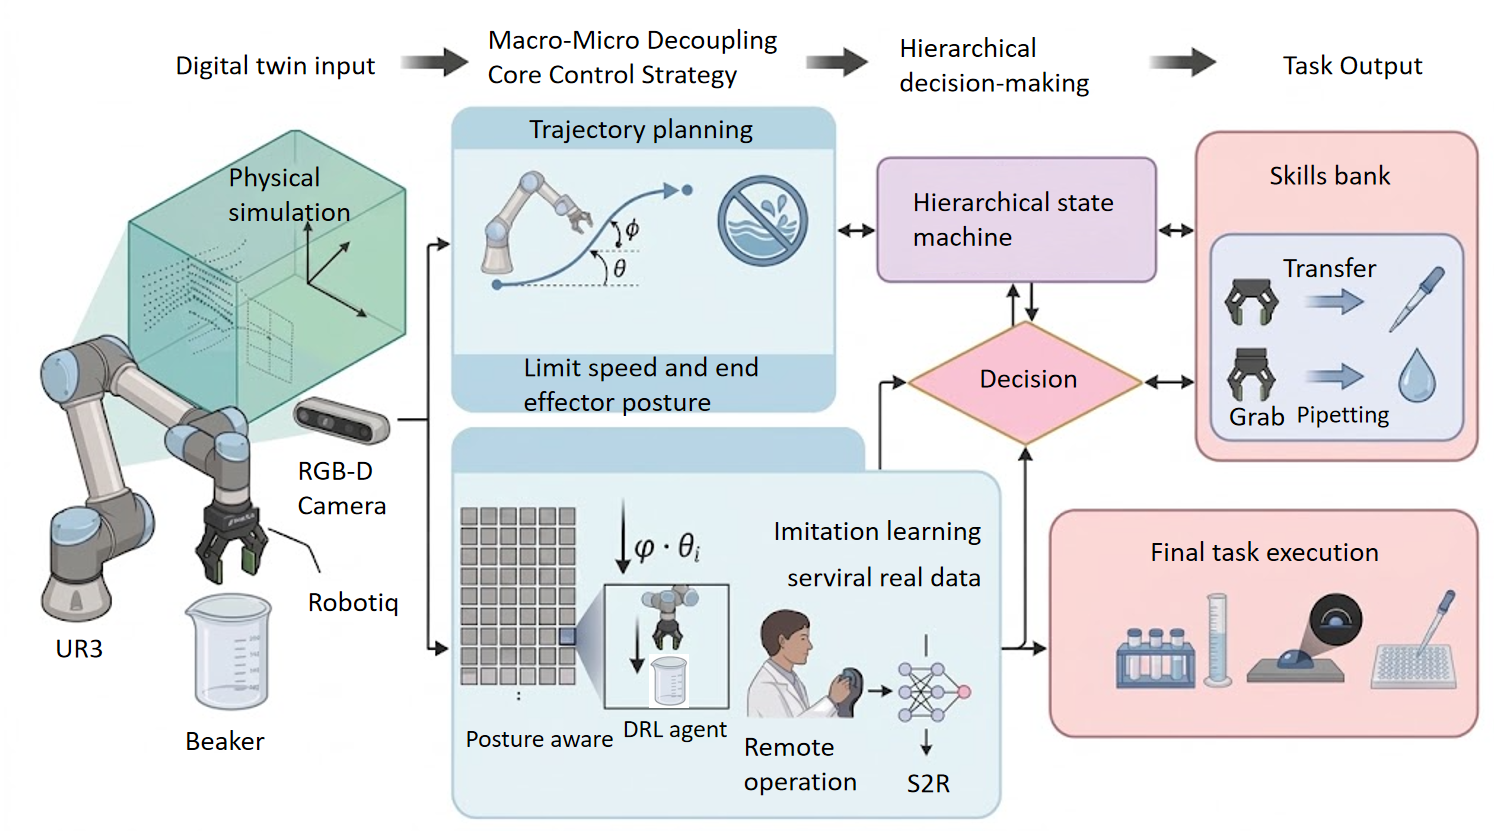
\includegraphics[width=\textwidth]{images/Framework.png}
    \caption{系统控制框架：结合物理仿真与RGB-D感知、约束轨迹规划、姿态感知强化学习、模仿学习与虚实迁移适配，并通过分层状态机调用可复用技能完成实验室任务。}
    \label{fig:overall_framework}
\end{figure*}

本章详细介绍了专为生化自动化化验（包括溶液配置、水滴角检测和梯度稀释）量身定制的多平台混合机器人框架。为了应对异构任务需求，跨工位宏观转移由约束感知经典规划执行，而灵巧的机械臂操作则由融合了大规模并行深度强化学习（DRL）与人在回路模仿学习（IL）的混合学习架构统筹。

\subsection{用于策略训练的仿真环境}
\label{subsec:simulation_training}

图~\ref{fig:simulation_overview}概括了环境构建、技能并行训练及物理部署过程。
\begin{figure*}[!t]
    \centering
    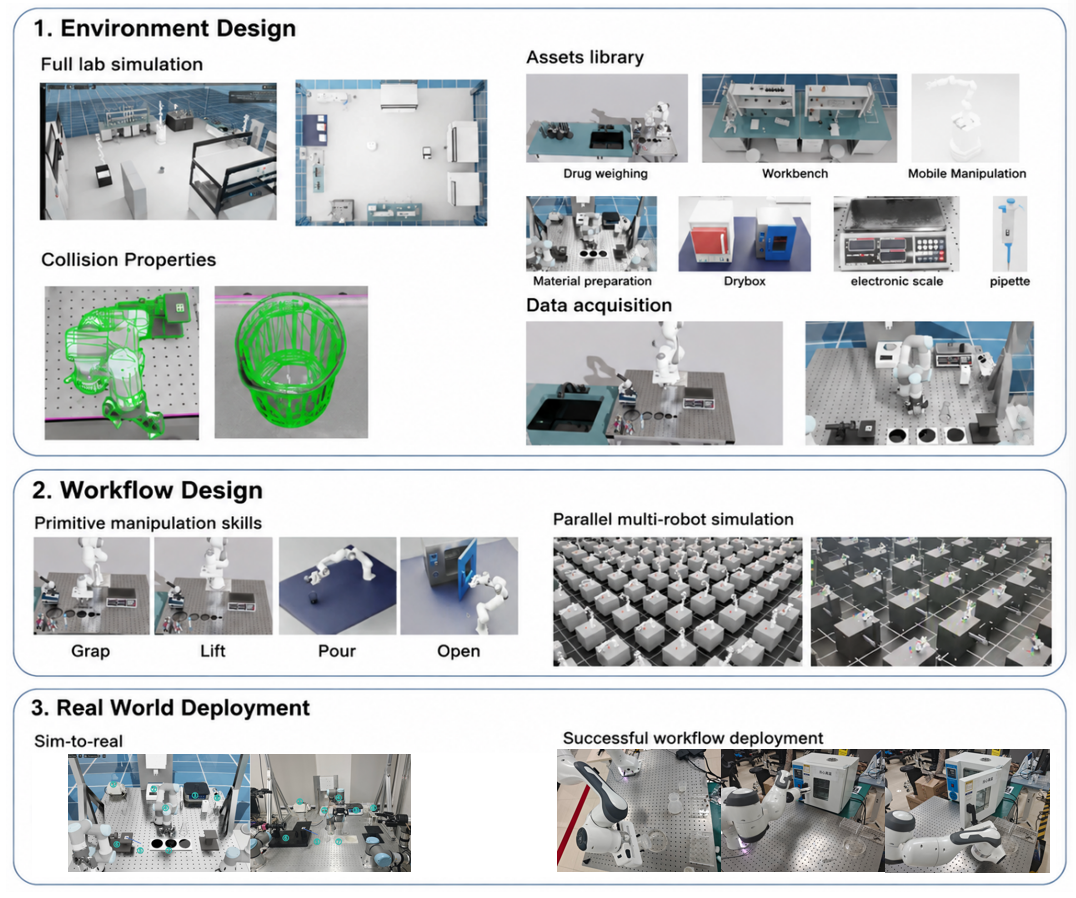
\includegraphics[width=0.94\textwidth]{images/environment_design2.png}
    \caption{仿真开发与物理部署总览：实验室环境与资产构建、碰撞建模和数据采集；操作技能开发与并行仿真；以及实验室操作的虚实迁移部署。}
    \label{fig:simulation_overview}
\end{figure*}

为了实现接触密集型任务的无风险训练与预验证，我们利用NVIDIA Isaac Sim构建了高保真仿真环境。在GPU加速张量物理引擎的驱动下，仿真环境能够准确建模刚体动力学、关节力矩和摩擦接触。夹爪和器材固定架均赋予了有符号距离场（SDF）碰撞网格，以实现无穿透的接触仿真。至关重要的是，独立的Python API架构实现了跨数千个并发虚拟环境的GPU并行化，彻底突破了物理机器人学习中样本效率低下的瓶颈。

\subsection{仿真环境与实体环境的状态同步}
\label{subsec:state_sync}

图~\ref{fig:state_sync_mechanism}展示坐标与时间对齐、观测有效性检查，以及带来源标记的虚拟实验台状态更新。
\begin{figure*}[!t]
    \centering
    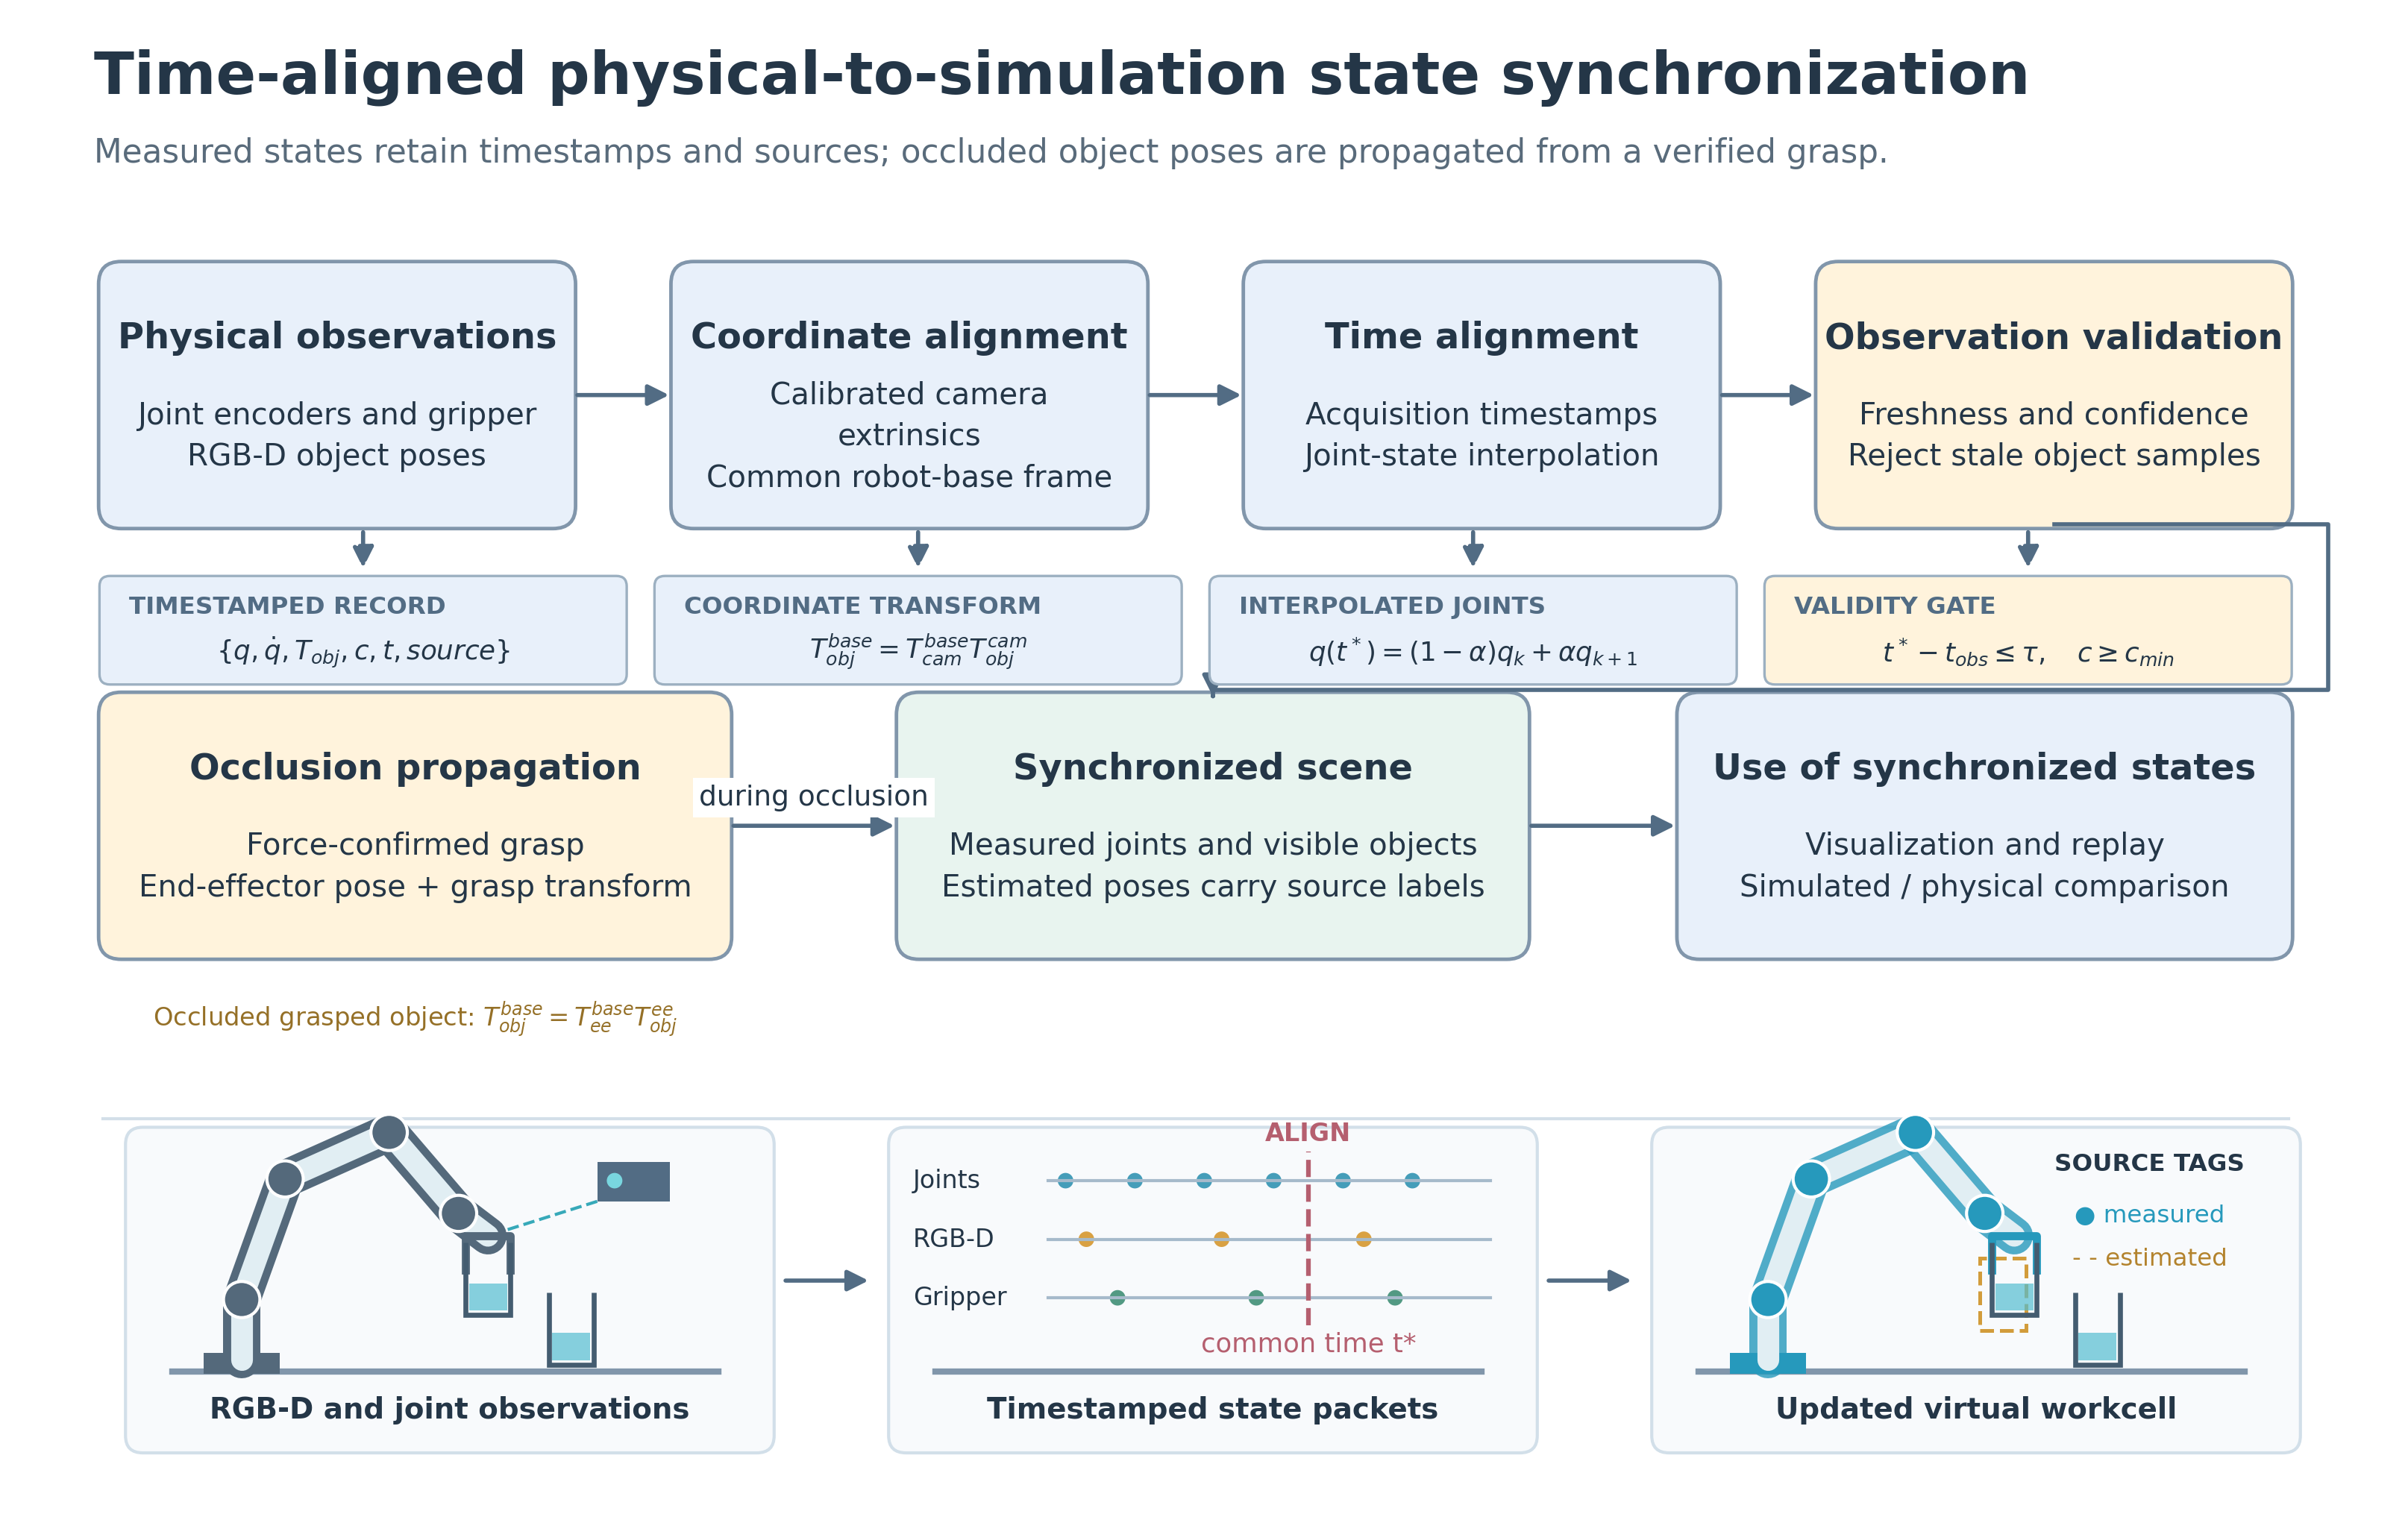
\includegraphics[width=\textwidth]{images/mechanisms/state_synchronization_mechanism.png}
    \caption{时间对齐的实体到仿真状态同步机制。异步关节、RGB-D与夹爪观测对齐到共同时间，并经有效性检查后更新场景。实线与虚线物体轮廓区分测量与传播估计位姿；同步用于可视化和比较，不代表已验证预测闭环控制。机械臂为示意绘制。}
    \label{fig:state_sync_mechanism}
\end{figure*}

我们定义实体机器人与Isaac Sim仿真环境之间的状态接口。关节编码器提供机械臂关节位置$\mathbf q_t$和速度$\dot{\mathbf q}_t$，夹爪提供开合状态与抓取确认信号；RGB-D视觉观测提供可见物体的位置$\mathbf p_{i,t}$、姿态$\mathbf R_{i,t}$及检测置信度。仅在连续观测可靠时估计物体速度。每条状态记录保留采集时间戳和数据来源，以区分直接测量与估计状态。

更新仿真场景前，利用标定外参将视觉观测转换到机器人基座坐标系，并将关节与物体观测对齐到共同时间戳。关节位置在相邻编码器采样之间插值；物体位姿由最近一次有效视觉观测更新。物体在力反馈确认抓取后短暂遮挡时，根据末端位姿和已估计的抓取变换传播其位姿。对过期或低置信度的物体观测不作为当前测量使用。同步后的状态用于可视化和比较仿真与实体轨迹；状态同步本身不能证明仿真预测精度或闭环控制性能。

\subsection{面向宏观导航的约束感知运动规划}
\label{subsec:macro_planning}

% \begin{figure}[htbp]
%     \centering
%     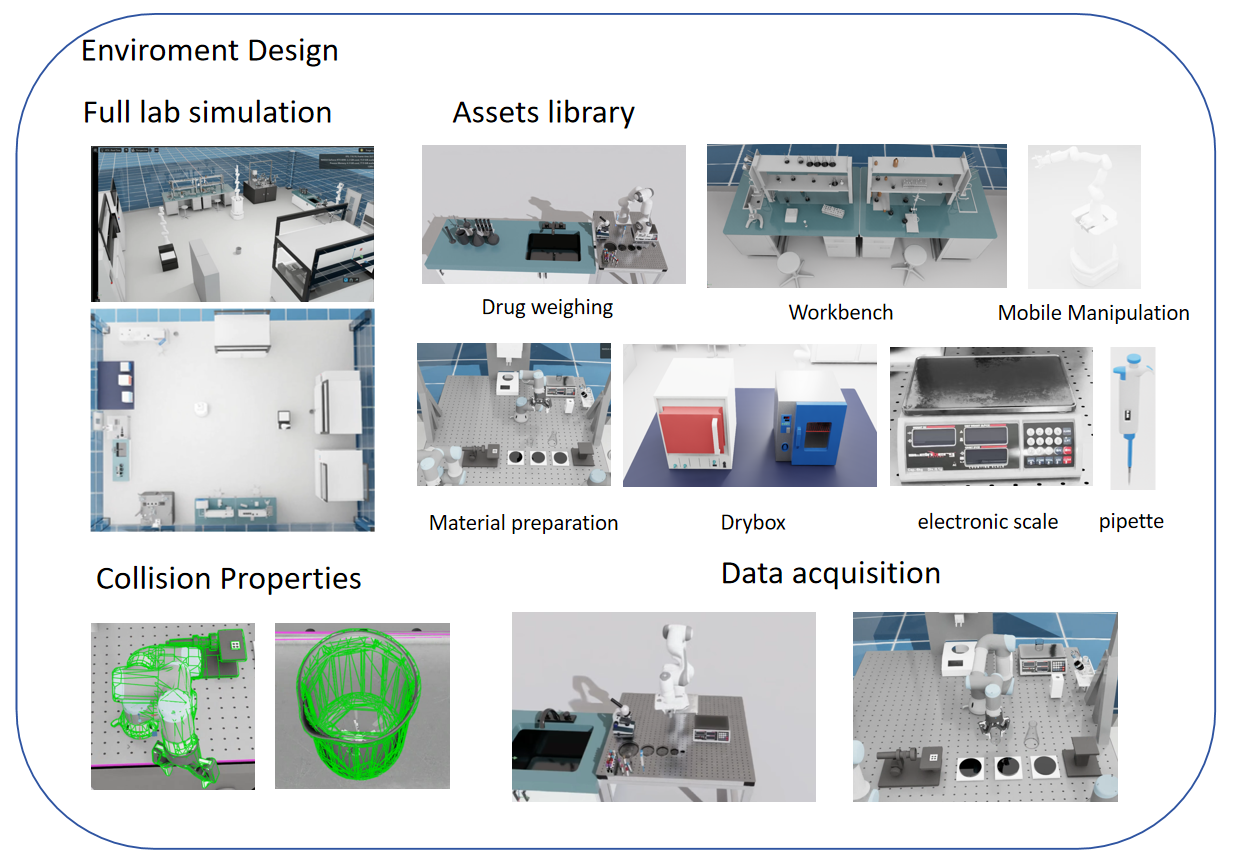
\includegraphics[width=0.9\linewidth]{images/environment_design.png}
%     \caption{基于Isaac Sim构建的高保真仿真环境。该仿真环境集成了UR3机械臂和Robotiq 2F-85平行夹爪，并采用有符号距离场（SDF）碰撞网格实现精确的接触建模。}
%     \label{fig:sim_env}
% \end{figure}

对于工作站之间的宏观转移（例如运送配好的试剂瓶），我们采用约束感知的经典运动规划器。为了防止移动过程中的流体晃动，对末端执行器的横滚角（$\phi$）和俯仰角（$\theta$）施加了严格的任务空间姿态约束：
\begin{equation}
    |\phi(t) - \phi_{\text{target}}| \leq \epsilon_{\phi}, \quad |\theta(t) - \theta_{\text{target}}| \leq \epsilon_{\theta}, \quad \forall t \in [0, T]
\end{equation}
路径平滑被公式化为最小冲击（minimum-jerk）轨迹优化问题：
\begin{equation}
    \min_{q(t)} \int_{0}^{T} \left\| \dddot{q}(t) \right\|^2 dt
\end{equation}
受关节速度（$\dot{q}_{\max}$）和加速度（$\ddot{q}_{\max}$）限制，保证了容器平稳、无碰撞的转移。

\subsection{带姿态感知奖励工程的大规模并行DRL}
\label{subsec:arm_rl}

对于实验器材的抓取与抬升，显式建模微观接触动力学在计算上是难以处理的。我们实施了公式化为马尔可夫决策过程（MDP）的深度强化学习（DRL）管线，定义为元组$\mathcal{M} = (\mathcal{S}, \mathcal{A}, \mathcal{P}, \mathcal{R}, \gamma)$：

\begin{itemize}
    \item \textbf{状态空间}$\mathcal{S}$：在每个时间步$t$，状态观测$s_t \in \mathcal{S}$由以下部分组成：
    \begin{equation}
        s_t = [\mathbf{q}_t, \dot{\mathbf{q}}_t, \mathbf{p}_{ee}, \mathbf{R}_{ee}, \mathbf{p}_{obj}, \mathbf{R}_{obj}, g_t]
    \end{equation}
    其中$\mathbf{q}_t \in \mathbb{R}^6$表示关节位置，$\dot{\mathbf{q}}_t \in \mathbb{R}^6$表示关节速度，$\mathbf{p}_{ee} \in \mathbb{R}^3$和$\mathbf{R}_{ee} \in SO(3)$表示末端执行器位姿，$\mathbf{p}_{obj} \in \mathbb{R}^3$和$\mathbf{R}_{obj} \in SO(3)$表示物体位姿，$g_t \in \{0, 1\}$是夹爪状态。

    \item \textbf{动作空间}$\mathcal{A}$：连续动作$a_t \in \mathcal{A}$由以下部分组成：
    \begin{equation}
        a_t = [\Delta\mathbf{q}_t, \Delta g_t] \in \mathbb{R}^7
    \end{equation}
    其中$\Delta\mathbf{q}_t \in \mathbb{R}^6$表示关节速度指令，$\Delta g_t \in [-1, 1]$控制夹爪开合。

    \item \textbf{转移动力学}$\mathcal{P}$：状态转移概率$\mathcal{P}(s_{t+1}|s_t, a_t)$由物理引擎仿真控制。

    \item \textbf{奖励函数}$\mathcal{R}$：奖励信号$r_t = \mathcal{R}(s_t, a_t)$设计用于引导策略成功抓取（详见第~\ref{subsec:reward_design}节）。

    \item \textbf{折扣因子}$\gamma \in [0, 1)$：平衡即时奖励和未来奖励。
\end{itemize}

MDP的目标是找到一个策略$\pi$，使得期望累积折扣奖励最大化：
\begin{equation}
    J(\pi) = \mathbb{E}_{\tau \sim \pi} \left[ \sum_{t=0}^{T} \gamma^t r_t \right]
\end{equation}
其中$\tau = (s_0, a_0, s_1, a_1, \dots)$表示从策略$\pi$采样的轨迹。

\subsubsection{价值函数与Bellman方程}
\label{subsec:bellman}

状态价值函数$V^\pi(s)$和动作价值函数$Q^\pi(s, a)$量化了在策略$\pi$下从状态$s$（并执行动作$a$）出发的期望回报：
\begin{align}
    V^\pi(s) &= \mathbb{E}_{\pi} \left[ \sum_{k=0}^{\infty} \gamma^k r_{t+k} \,\Big|\, s_t = s \right] \\
    Q^\pi(s, a) &= \mathbb{E}_{\pi} \left[ \sum_{k=0}^{\infty} \gamma^k r_{t+k} \,\Big|\, s_t = s, \, a_t = a \right]
\end{align}

这些价值函数满足递归Bellman方程：
\begin{align}
    V^\pi(s) &= \mathbb{E}_{a \sim \pi} \left[ \mathcal{R}(s, a) + \gamma \, V^\pi(s') \right] \\
    Q^\pi(s, a) &= \mathcal{R}(s, a) + \gamma \, \mathbb{E}_{s' \sim \mathcal{P}} \left[ V^\pi(s') \right]
\end{align}

最优价值函数满足Bellman最优方程：
\begin{align}
    V^*(s) &= \max_{a} \left[ \mathcal{R}(s, a) + \gamma \, \mathbb{E}_{s' \sim \mathcal{P}} \left[ V^*(s') \right] \right] \\
    Q^*(s, a) &= \mathcal{R}(s, a) + \gamma \, \mathbb{E}_{s' \sim \mathcal{P}} \left[ \max_{a'} Q^*(s', a') \right]
\end{align}

优势函数$A^\pi(s, a)$用于衡量动作$a$相对于策略平均水平的优劣：
\begin{equation}
    A^\pi(s, a) = Q^\pi(s, a) - V^\pi(s)
\end{equation}

\subsubsection{策略梯度定理}
\label{subsec:policy_gradient}

策略梯度定理为优化参数化策略$\pi_\theta$提供了理论基础。目标函数$J(\theta)$关于策略参数$\theta$的梯度为：
\begin{equation}
    \nabla_\theta J(\theta) = \mathbb{E}_{\tau \sim \pi_\theta} \left[ \sum_{t=0}^{T} \nabla_\theta \log \pi_\theta(a_t | s_t) \, A^{\pi_\theta}(s_t, a_t) \right]
\end{equation}

实际中，优势函数通过时序差分（TD）误差估计：
\begin{equation}
    \delta_t = r_t + \gamma V_\phi(s_{t+1}) - V_\phi(s_t)
\end{equation}
其中$V_\phi$是参数为$\phi$的学习价值函数（评论家）。


\subsubsection{奖励函数设计}
\label{subsec:reward_design}

为了防止抓取过程中液体容器倾斜，我们设计了带有\textit{姿态感知乘数}的密集奖励函数。设$\mathbf{z}_{\text{curr}}$为物体的归一化局部z轴向量，$\mathbf{z}_{\text{target}} = [0, 0, -1]^T$为理想的向下重力向量。姿态乘数$M_{\text{posture}}$定义为：
\begin{equation}
    M_{\text{posture}} = \text{clamp}(\mathbf{z}_{\text{curr}} \cdot \mathbf{z}_{\text{target}}, \, 0.0, \, 1.0)
\end{equation}

每个时间步的完整奖励函数由多个分量组成：
\begin{equation}
    R_t = \underbrace{R_{\text{distance}}}_{\text{靠近}} + \underbrace{R_{\text{grasp}}}_{\text{抓取}} + \underbrace{R_{\text{lift}}}_{\text{抬升}} - \underbrace{R_{\text{collision}}}_{\text{惩罚}}
\end{equation}

其中各分量定义如下：
\begin{align}
    R_{\text{distance}} &= -\alpha_1 \left\| \mathbf{p}_{ee} - \mathbf{p}_{obj} \right\|_2 \cdot M_{\text{posture}} \\
    R_{\text{grasp}} &= \alpha_2 \cdot \mathbb{I}[\text{grasped}] \cdot M_{\text{posture}} \\
    R_{\text{lift}} &= \alpha_3 \cdot (z_{obj} - z_{obj,0}) \cdot M_{\text{posture}} \\
    R_{\text{collision}} &= \alpha_4 \cdot \mathbb{I}[\text{collision}]
\end{align}

其中$\alpha_1, \alpha_2, \alpha_3, \alpha_4$为权重系数，$\mathbb{I}[\cdot]$为指示函数，$z_{obj,0}$为物体初始高度。若容器倾斜超过$90^\circ$，$M_{\text{posture}}$衰减为零，重度惩罚不当姿态，迫使策略掌握直立抓取。

\subsubsection{熵正则化目标}
\label{subsec:entropy}

为了鼓励探索并防止策略过早收敛到次优解，我们采用熵正则化的RL目标。策略$\pi_\theta$在状态$s$处的熵定义为：
\begin{equation}
    \mathcal{H}[\pi_\theta](s) = -\mathbb{E}_{a \sim \pi_\theta(\cdot|s)} \left[ \log \pi_\theta(a | s) \right]
\end{equation}

对于具有高斯策略$\pi_\theta(a|s) = \mathcal{N}(\mu_\theta(s), \Sigma_\theta(s))$的连续动作空间，熵具有解析形式：
\begin{equation}
    \mathcal{H}[\pi_\theta] = \frac{1}{2} \log \left( (2\pi e)^k \det(\Sigma_\theta) \right)
\end{equation}
其中$k$为动作维度。最大熵目标在标准RL目标基础上增加了熵正则项：
\begin{equation}
    J_{\text{ME}}(\theta) = \mathbb{E}_{\tau \sim \pi_\theta} \left[ \sum_{t=0}^{T} \gamma^t \left( r_t + \alpha \mathcal{H}[\pi_\theta](s_t) \right) \right]
\end{equation}
其中$\alpha > 0$为温度参数，控制探索-利用的权衡。

\subsubsection{PPO优化}
\label{subsec:ppo}

在Isaac Sim中分布于4,096个并行虚拟环境中的近端策略优化（PPO）算法加速了训练。PPO裁剪代理目标定义为：
\begin{equation}
    L^{CLIP}(\theta) = \hat{\mathbb{E}}_t \left[ \min \left( r_t(\theta) \hat{A}_t, \, \text{clip}(r_t(\theta), 1-\epsilon, 1+\epsilon) \hat{A}_t \right) \right]
\end{equation}

其中$r_t(\theta) = \frac{\pi_\theta(a_t|s_t)}{\pi_{\theta_{old}}(a_t|s_t)}$为概率比，$\hat{A}_t$为使用广义优势估计（GAE）计算的估计优势函数：
\begin{equation}
    \hat{A}_t = \sum_{l=0}^{T-t} (\gamma \lambda)^l \delta_{t+l}, \quad \delta_t = r_t + \gamma V(s_{t+1}) - V(s_t)
\end{equation}

总损失函数结合了裁剪代理、价值函数和熵奖励：
\begin{equation}
    L(\theta) = L^{CLIP}(\theta) - c_1 L^{VF}(\theta) + c_2 H[\pi_\theta](s_t)
\end{equation}

其中$L^{VF} = (V_\theta(s_t) - V_t^{\text{target}})^2$为价值函数损失，$H[\pi_\theta]$为鼓励探索的熵奖励，$c_1, c_2$为系数。

训练超参数总结于表~\ref{tab:hyperparameters}。

\begin{table}[!t]
\renewcommand{\arraystretch}{1.3}
\caption{PPO训练超参数}
\label{tab:hyperparameters}
\centering
\begin{tabular}{lc}
\hline\hline
\textbf{超参数} & \textbf{数值} \\ \hline
学习率 & $3 \times 10^{-4}$ \\
折扣因子$\gamma$ & 0.99 \\
GAE参数$\lambda$ & 0.95 \\
裁剪参数$\epsilon$ & 0.2 \\
熵系数$c_2$ & 0.01 \\
价值损失系数$c_1$ & 0.5 \\
批次大小 & 4096 \\
小批次大小 & 512 \\
每次更新轮数 & 10 \\
最大梯度范数 & 0.5 \\
并行环境数量 & 4096 \\
训练迭代次数 & 5000 \\ \hline\hline
\end{tabular}
\end{table}

\subsubsection{域随机化}
\label{subsec:domain_randomization}

为了弥合虚实差距，我们在训练过程中应用了广泛的域随机化。随机化参数$\theta_{DR}$从均匀分布中采样：
\begin{equation}
    \theta_{DR} \sim \mathcal{U}(\theta_{\text{base}} - \Delta\theta, \, \theta_{\text{base}} + \Delta\theta)
\end{equation}

具体的随机化范围详见表~\ref{tab:domain_randomization}。

\begin{table}[!t]
\renewcommand{\arraystretch}{1.3}
\caption{域随机化参数}
\label{tab:domain_randomization}
\centering
\begin{tabular}{lcc}
\hline\hline
\textbf{参数} & \textbf{基准值} & \textbf{范围} \\ \hline
桌面摩擦系数 & 0.5 & $[0.3, 0.8]$ \\
物体质量 (g) & 100 & $[80, 130]$ \\
夹爪摩擦系数 & 0.8 & $[0.5, 1.2]$ \\
光照强度 & 1.0 & $[0.6, 1.4]$ \\
相机位置 (cm) & -- & $\pm 5$ \\
物体位置 (cm) & -- & $\pm 3$ \\ \hline\hline
\end{tabular}
\end{table}

为了进一步增强所学策略的鲁棒性，我们在随机化边界上应用了结构化的课程学习。域随机化范围$\Delta\theta$在训练过程中逐步扩展：
\begin{equation}
    \Delta\theta^{(k)} = \Delta\theta_{\min} + \left( \Delta\theta_{\max} - \Delta\theta_{\min} \right) \cdot \sigma\!\left( \frac{k - k_{\text{mid}}}{k_{\text{scale}}} \right)
\end{equation}
其中$k$为当前训练迭代次数，$\sigma(\cdot)$为sigmoid函数，$k_{\text{mid}}$和$k_{\text{scale}}$控制课程调度。这确保智能体首先在轻微扰动下掌握任务，然后再面对完整的随机化范围。

\subsubsection{多步回报}
\label{subsec:multi_step}

为了减少单步TD估计的偏差并加速信用分配，我们采用$n$步回报进行价值函数自举。$n$步回报$G_t^{(n)}$定义为：
\begin{equation}
    G_t^{(n)} = \sum_{k=0}^{n-1} \gamma^k r_{t+k} + \gamma^n V_\phi(s_{t+n})
\end{equation}

广义形式通过加权平均组合所有$n$步回报（用于GAE）：
\begin{equation}
    G_t^{\text{GAE}(\gamma, \lambda)} = (1 - \lambda) \sum_{n=1}^{\infty} \lambda^{n-1} G_t^{(n)}
\end{equation}
其中$\lambda \in [0, 1]$在高偏差低方差（$\lambda \to 0$）和低偏差高方差（$\lambda \to 1$）估计之间进行插值。

\subsection{模仿学习与少样本虚实迁移微调}
\label{subsec:arm_il_adaptation}

图~\ref{fig:sim_to_real_mechanism}概括基于行为克隆的迁移流程，包括随机化仿真示教、正则化适配及独立实体测试。
\begin{figure*}[!t]
    \centering
    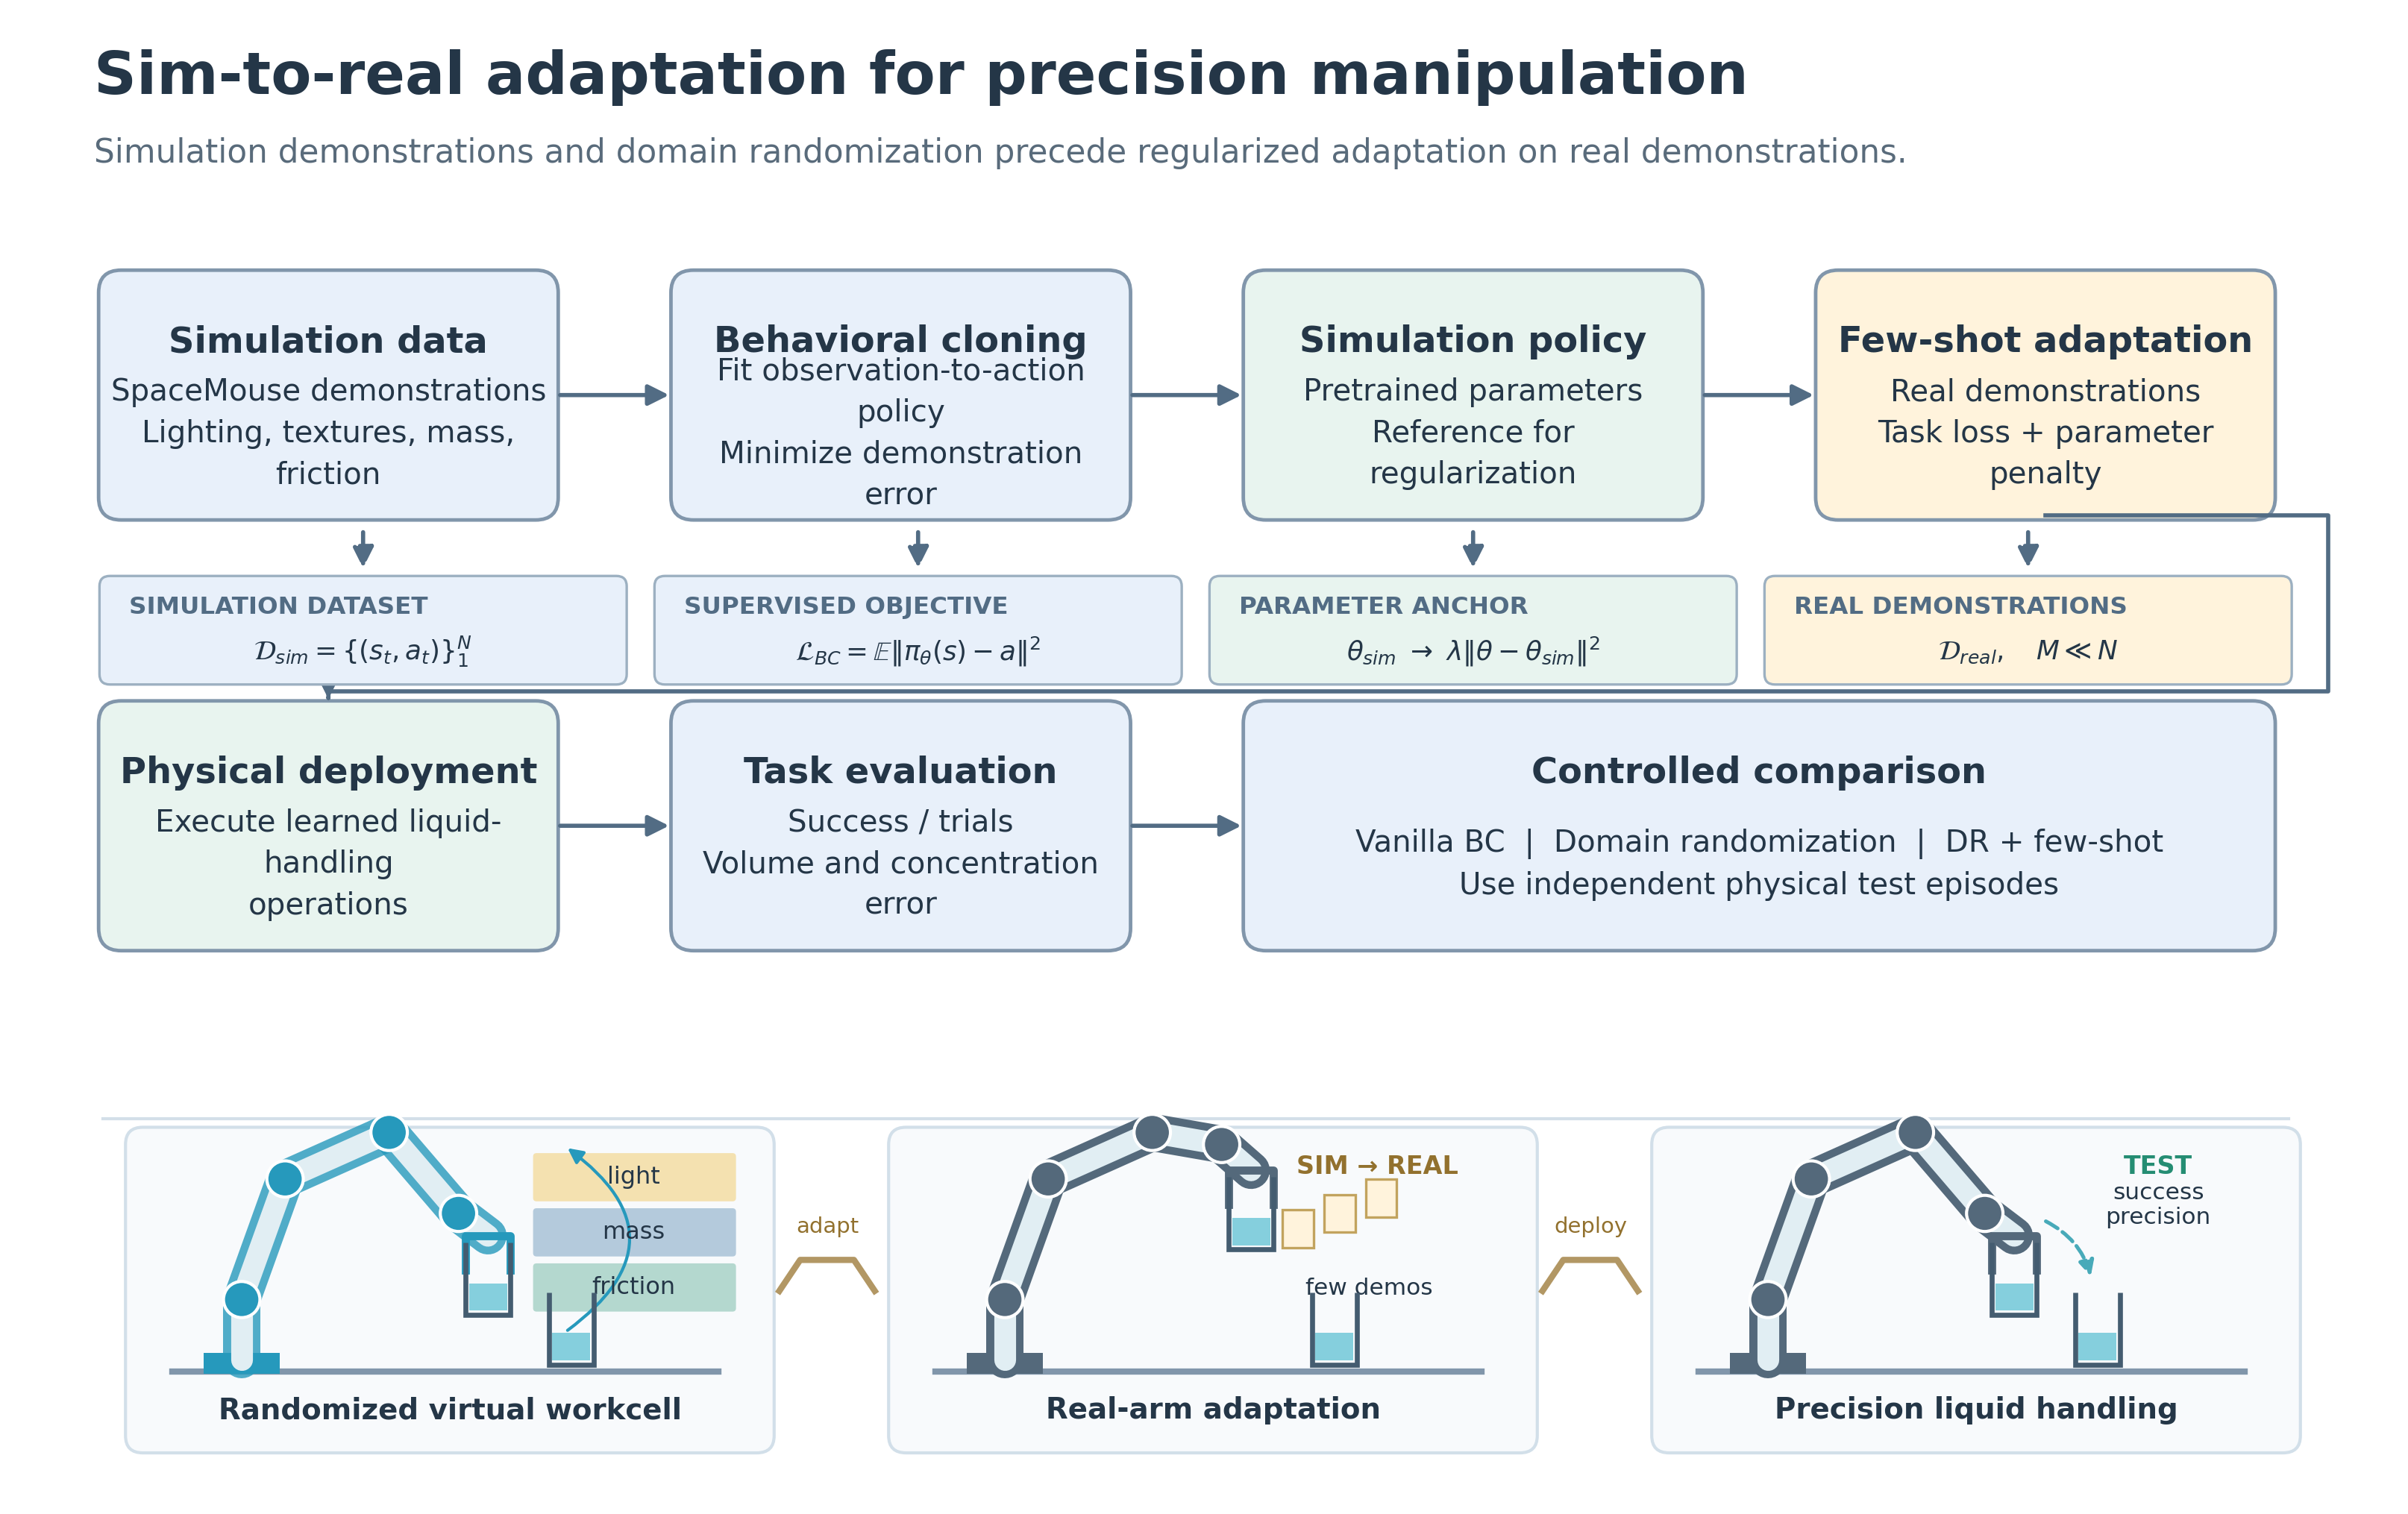
\includegraphics[width=\textwidth]{images/mechanisms/sim_to_real_mechanism.png}
    \caption{精密操作的虚实迁移机制。行为克隆与域随机化提供仿真策略，少量实体示教用于带参数正则化的微调。桥梁示意适配与部署，对比模块表示评估方案而非额外训练步骤。机械臂为示意绘制。}
    \label{fig:sim_to_real_mechanism}
\end{figure*}

对于微量移液和液滴滴加等精度要求极高的微观操作，我们引入了遥操作引导的模仿学习（IL）管线。利用6自由度SpaceMouse接口在仿真中采集专家示教数据$\mathcal{D}_{\text{sim}} = \{(s_t, a_t)\}_{i=1}^N$，并通过行为克隆（BC）预训练视觉运动策略$\pi_\theta(a_t | s_t)$：
\begin{equation}
    \mathcal{L}_{\text{BC}}(\theta) = \mathbb{E}_{(s_t, a_t) \sim \mathcal{D}_{\text{sim}}} \left[ \left\| \pi_\theta(s_t) - a_t \right\|_2^2 \right]
\end{equation}
仿真训练期间应用了包含光照、纹理、物体质量和摩擦系数的域随机化（DR）。

为了弥合由液体表面张力、光学折射和夹爪柔顺形变引起的真实世界虚实鸿沟，我们利用极少量（$M$组）物理示教实施了带正则化的少样本真实世界微调机制。策略参数通过最小化以下目标自适应调整为$\theta_{\text{real}}$：
\begin{equation}
    \theta_{\text{real}} = \arg\min_{\theta} \left( \mathbb{E}_{(s_t, a_t) \sim \mathcal{D}_{\text{real}}} \left[ \left\| \pi_\theta(s_t) - a_t \right\|_2^2 \right] + \lambda \left\| \theta - \theta_{\text{sim}} \right\|_2^2 \right)
\end{equation}
其中$\lambda$为正则化超参数，防止对仿真学到特征的灾难性遗忘，实现了鲁棒的物理部署。

为了缓解行为克隆固有的分布偏移问题，我们还采用了DAgger（数据集聚合）方法，该方法在学习者自身的状态分布下迭代采集纠正示教：
\begin{equation}
    \mathcal{D}_{\text{DAgger}} = \mathcal{D}_{\text{sim}} \cup \left\{ \left( s_t^{\pi_\theta}, \, a_t^{\text{expert}} \right) \right\}_{t=1}^{T}
\end{equation}
其中$s_t^{\pi_\theta}$为当前策略访问的状态，$a_t^{\text{expert}}$为专家纠正动作。聚合数据集用于重新训练策略，逐步减少复合误差。

此外，对于需要多模态动作分布的任务，我们引入了受GAIL \cite{ho2016gail}启发的基于判别器的对抗损失：
\begin{equation}
    \min_{\theta} \max_{\omega} \; \mathbb{E}_{\pi_\theta} \left[ \log D_\omega(s, a) \right] + \mathbb{E}_{\mathcal{D}_{\text{expert}}} \left[ \log(1 - D_\omega(s, a)) \right] - \lambda_{\text{ent}} \mathcal{H}[\pi_\theta]
\end{equation}
其中$D_\omega$为学习到的判别器，用于区分专家生成和策略生成的状态转移，$\lambda_{\text{ent}}$为熵奖励系数。

\subsection{具备失败恢复机制的分层状态机与技能库}
\label{subsec:hierarchical_skill}

图~\ref{fig:hsm_recovery_mechanism}展示基于条件的技能编排，以及验证失败后的有限次数恢复。
\begin{figure*}[!t]
    \centering
    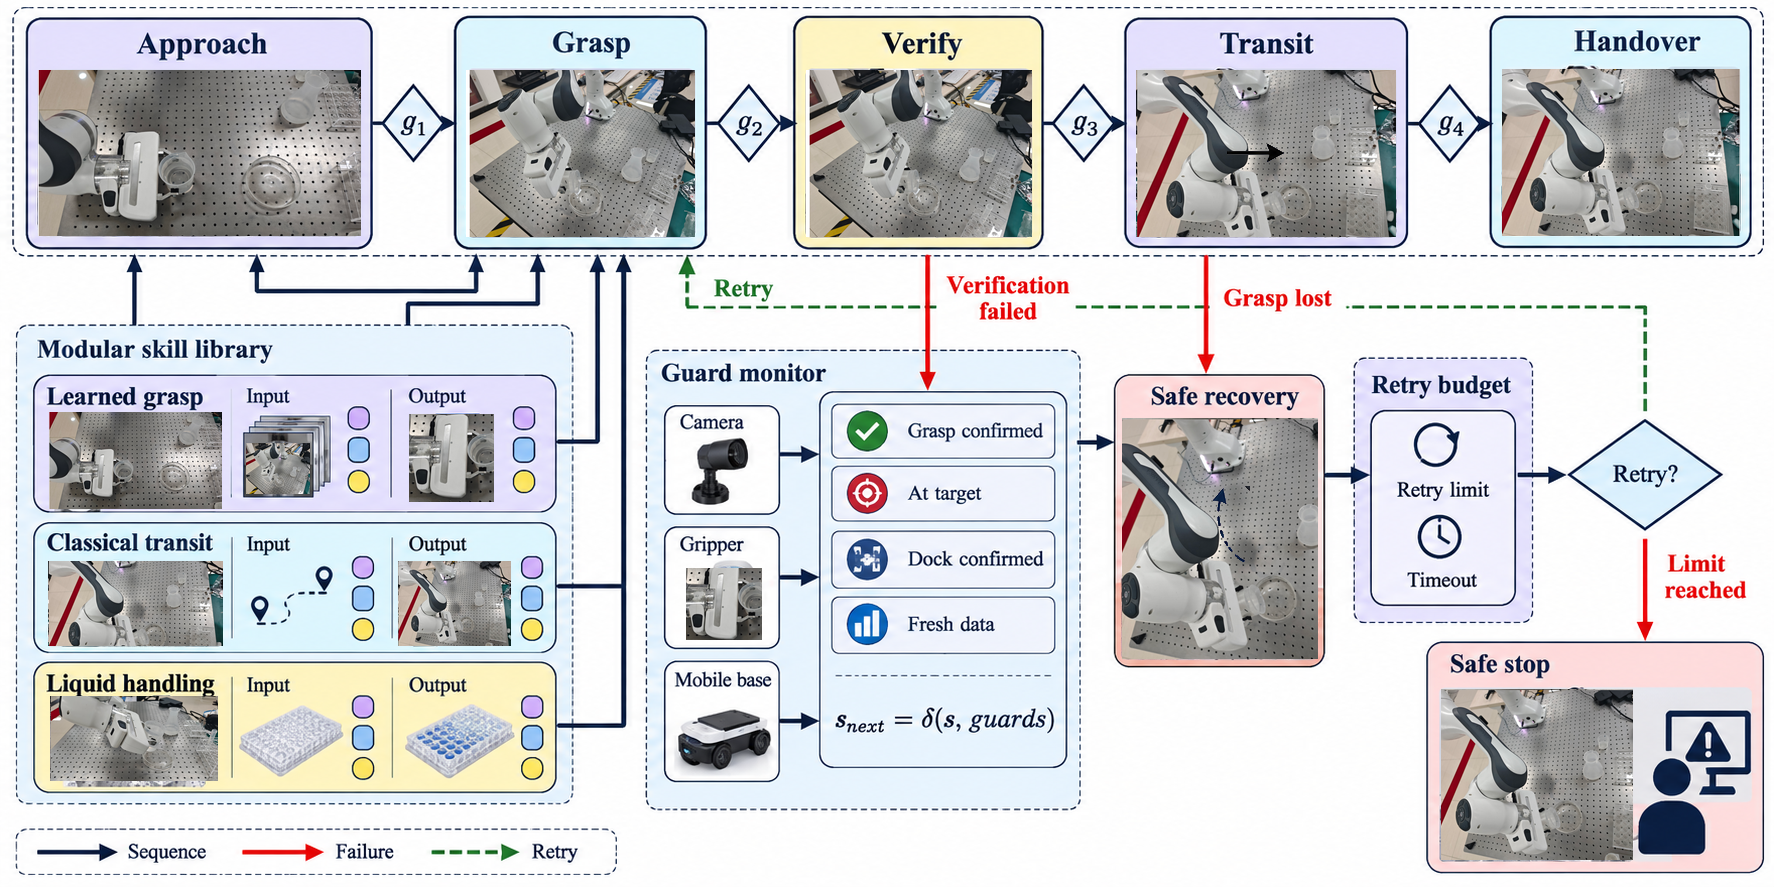
\includegraphics[width=\textwidth]{images/mechanisms/hsm_recovery_reference_style_panda_photos.png}
    \caption{具备失败恢复机制的分层状态机与模块化技能库。完成条件允许顺序推进，验证失败或抓取丢失触发有限安全恢复，达到重试或超时上限则安全停止。Panda画面直接裁剪自原始实验照片并复用于设备示意，不是交接或恢复阶段的独立实验证据；其余图标为示意，不表示经训练的高层策略或已测得的恢复收益。}
    \label{fig:hsm_recovery_mechanism}
\end{figure*}

为协调抓取、转移和移液等多阶段任务，我们在模块化\textit{技能库}之上采用规则驱动的分层状态机（HSM）。上层任务编排不是经训练的强化学习策略；其作用是将任务顺序、状态转移和失败恢复条件显式定义。

技能库$\mathcal{L}_{\text{skills}} = \{\pi_{\text{grasp}}, \pi_{\text{transit}}, \pi_{\text{pour}}, \dots\}$包含独立实现的操作策略及经典规划程序。每个技能规定前置条件、完成判据、超时限制和失败代码。模块化允许单独更新某一技能，但若无与单体策略的对照实验，不能宣称已消除负迁移。

状态机包含\texttt{approach}、\texttt{grasp}、\texttt{verify}、\texttt{transit}、\texttt{handover}和\texttt{recover}等状态。预定义条件检查\texttt{is\_bottle\_grasped}、\texttt{is\_at\_target}、对接确认和传感器数据新鲜度。给定当前状态与条件结果，转移$s_{t+1}=\delta(s_t,g(o_t))$是确定性的；本文不假设状态转移概率或学习得到的置信度。


若抓取验证失败，状态机停止转移，并在安全重新定位后返回\texttt{grasp}。重试次数与超时限制约束重复尝试；达到上限则进入安全停止状态，等待人工检查。这是所定义的恢复机制，不等于已经证实恢复率提升。应与无恢复机制的固定顺序状态机比较，报告阶段及完整工作流成功率、恢复次数、人工干预次数和完成时间。

\section{实验与结果}
\label{sec:experiments}

在本节中，我们进行了广泛的实证评估，以验证所提出的多平台混合框架。实验旨在验证四个核心假设：1）约束感知的宏观规划器是否能有效防止液体溢出；2）姿态感知的大规模并行DRL智能体是否能保证直立器材抓取；3）正则化少样本微调管线是否能成功弥合基于IL的微量移液的虚实鸿沟；4）完整系统是否能无缝地端到端自主执行生化化验工作流。

对具有成功次数与试验次数的二元结果，使用Wilson得分法计算95\%置信区间：
\begin{equation}
    \begin{aligned}
    D &= 1+z^2/n,\quad z=1.96,\\
    c &= (\hat p+z^2/(2n))/D,\\
    h &= \frac{z}{D}\sqrt{\frac{\hat p(1-\hat p)}{n}+\frac{z^2}{4n^2}},\\
    \text{CI}_{95\%} &= [c-h,c+h].
    \end{aligned}
\end{equation}
其中$\hat{p}$为观测成功率，$n$为实验次数。
连续指标应在独立样品或回合层面估计不确定性。若无原始配对记录，不能仅凭汇总百分比宣称统计显著。

\subsection{实验平台与硬件配置}
\label{subsec:exp_setup}

物理验证平台严格镜像了Isaac Sim仿真环境。移动操作系统配备了一个差速驱动底盘和一个6自由度UR3机械臂。Robotiq 2F-85平行夹爪安装了定制的柔性橡胶垫，用于固定易碎的玻璃器皿和微孔板。

感知子系统方面，Intel RealSense D435 RGB-D相机以eye-to-hand构型安装，提供连续的点云和视觉反馈。计算管线——包括实时3D体素代价地图生成、DRL策略推理和分层状态机（HSM）序列控制——在本地NVIDIA RTX 4090工作站上执行，通过ROS桥接确保低延迟通信。

\subsection{状态同步实测结果}
\label{subsec:state_sync_eval}
表~\ref{tab:sync_illustrative}列出用户提供的仿真与实体状态接口实测汇总值。按所列汇总值，关节状态一致性、物体位姿误差、更新延迟、观测有效性和抓取状态识别均满足预设目标。物体位姿误差应以独立参考测量计算，不能以更新仿真场景的同一RGB-D估计作为真值。目前尚未获得对应的回合数、原始时间戳轨迹、参考测量方法和不确定性区间，故这些汇总值仍需逐回合记录核验，不能据此进行统计显著性判断。下文任务成功率来自其他实验，不应视为状态同步指标。

\begin{table}[!t]
\caption{状态同步目标与提供的实测汇总结果}
\label{tab:sync_illustrative}
\centering
\resizebox{\columnwidth}{!}{%
\begin{tabular}{lcc}
\hline\hline
\textbf{指标} & \textbf{目标} & \textbf{实测结果} \\ \hline
关节角度平均绝对误差 & $\leq 0.5^\circ$ & $0.42^\circ$ \\
关节角度误差95分位数 & $\leq 1.5^\circ$ & $1.2^\circ$ \\
物体位置误差：静止 & $\leq 3$ mm & $2.2$ mm \\
物体位置误差：运动 & $\leq 5$ mm & $3.4$ mm \\
物体位置误差：短暂遮挡 & $\leq 10$ mm & $8.1$ mm \\
物体姿态误差：运动 & $\leq 4^\circ$ & $3.6^\circ$ \\
更新延迟：中位数/95分位数 & $\leq 50/100$ ms & $41/87$ ms \\
过期或被拒绝观测比例 & $\leq 2\%$ & $1.4\%$ \\
抓取状态识别准确率 & $\geq 98\%$ & $98.7\%$ \\ \hline\hline
\end{tabular}}
\end{table}

\subsection{宏观导航与流体稳定性}
\label{subsec:exp_macro_benchmarks}

为评估宏观安全性，移动底盘被要求在高度杂乱的实验室环境中运输开敞液体容器。我们将本文的约束感知经典规划器与标准RRT*规划器和纯DRL导航策略进行了基准对比。评估指标包括整体成功率、最小障碍间距和平均轨迹冲击（流体晃动的主要指标）。

轨迹平滑度通过平均冲击指标量化：
\begin{equation}
    J_{\text{smooth}} = \frac{1}{T} \sum_{t=1}^{T} \left\| \dddot{\mathbf{q}}_t \right\|^2
\end{equation}
其中$\dddot{\mathbf{q}}_t$是时间步$t$处关节轨迹的三阶导数（冲击）。

\begin{table}[!t]
\renewcommand{\arraystretch}{1.3}
\caption{宏观导航规划器的定量比较}
\label{tab:navigation_metrics}
\centering
\begin{tabular}{lccc}
\hline\hline
\textbf{评估指标} & \textbf{标准RRT*} & \textbf{纯DRL} & \textbf{本文方法} \\ \hline
实验次数 / 成功次数 & 50\,/\,37 & 50\,/\,34 & 50\,/\,\textbf{44} \\
成功率 (\%) & 74.0 & 68.0 & \textbf{88.0} \\
Wilson 95\%区间 (\%) & [60.4,84.1] & [54.2,79.2] & [76.2,94.4] \\
平均轨迹冲击 ($m/s^3$) & 4.52 & 6.18 & \textbf{0.85} \\
最小间距 ($m$) & 0.12 & 0.08 & \textbf{0.28} \\
规划时间 (ms) & 12.3 & \textbf{2.1} & 8.7 \\ \hline\hline
\end{tabular}
\end{table}

表\ref{tab:navigation_metrics}支持本文规划器轨迹加加速度较低的结论，但不能单独证明液体不溢出。真实液体测试应在匹配容器、液体、填充率和路线的条件下，测量运输前后容器与托盘质量（同时控制蒸发和操作损失）、标定侧视相机得到的最大自由液面倾角，以及超过预定溢出阈值的回合比例；需覆盖正常行驶、转弯、急停和遇障重规划。目前这些直接液体测量值尚未提供。

\begin{table}[!t]
\caption{真实液体稳定性结果（待填）}
\label{tab:liquid_stability}
\centering
\begin{tabular}{lccc}
\hline\hline
\textbf{规划器} & \textbf{损失质量(g)} & \textbf{最大液面角} & \textbf{溢出次数/$n$} \\ \hline
RRT* & 待填 & 待填 & 待填 \\
纯DRL & 待填 & 待填 & 待填 \\
约束感知规划 & 待填 & 待填 & 待填 \\ \hline\hline
\end{tabular}
\end{table}

\subsection{面向姿态感知抓取的大规模并行DRL}
\label{subsec:exp_rl_grasping}

抓取未密封的液体药瓶是一项极具挑战的任务，因为在抬升阶段任何显著的倾斜都会导致化验失效。我们评估了在Isaac Sim中训练的大规模并行PPO抓取策略，并进行了消融实验，以单独验证本文提出的"姿态感知乘数（$M_{\text{posture}}$）"的贡献。我们将基线PPO（仅使用标准距离奖励训练）与本文的姿态感知PPO进行了对比。

\begin{table}[!t]
\renewcommand{\arraystretch}{1.3}
\caption{DRL姿态感知奖励机制的消融研究}
\label{tab:rl_grasping}
\centering
\begin{tabular}{lcc}
\hline\hline
\textbf{评估指标} & \textbf{基线PPO} & \textbf{姿态感知PPO} \\ \hline
实验次数 / 成功次数 & 200\,/\,158 & 200\,/\,\textbf{172} \\
抓取成功率 (\%) & 79.0 & \textbf{86.0} \\
Wilson 95\%区间 (\%) & [72.8,84.1] & [80.5,90.1] \\
最大倾斜角 (度) & $35.4^\circ \pm 12.1^\circ$ & $\mathbf{4.2^\circ \pm 1.5^\circ}$ \\
液体溢出率 (\%) & 42.0 & \textbf{0.0} \\
收敛迭代次数 & 8500 & \textbf{5000} \\ \hline\hline
\end{tabular}
\end{table}

表\ref{tab:rl_grasping}的结果凸显了显著的性能提升。基线PPO为了最小化轨迹距离，经常以激进的角度接近药瓶，导致平均抓取倾斜角高达$35.4^\circ$，泼洒率高达42.0\%。通过集成点积姿态乘数，我们的策略成功收敛至严格的垂直"自上而下（top-down）"抓取，将最大倾斜角锐减至仅仅$4.2^\circ$，并在零样本（zero-shot）物理真机部署期间彻底消除了液体泼洒现象。

\subsubsection{姿态权重敏感性分析}
\label{subsec:sensitivity_analysis}

为了研究姿态感知奖励权重的影响，我们通过将姿态乘数系数$\alpha_{\text{posture}}$从0.0变化到1.0来进行敏感性分析。如表\ref{tab:sensitivity}所示，增加$\alpha_{\text{posture}}$显著降低了倾斜角，但由于行为过于保守，可能会略微降低抓取成功率。

\begin{table}[!t]
\renewcommand{\arraystretch}{1.3}
\caption{姿态权重$\alpha_{\text{posture}}$的敏感性分析}
\label{tab:sensitivity}
\centering
\resizebox{\columnwidth}{!}{
\begin{tabular}{lcccc}
\hline\hline
\textbf{$\alpha_{\text{posture}}$} & \textbf{实验/成功} & \textbf{成功率 (\%)} & \textbf{倾斜角 ($^\circ$)} & \textbf{溢出率 (\%)} \\ \hline
0.0 & 200\,/\,162 & 81.0 & $38.5 \pm 14.2$ & 45.0 \\
0.2 & 200\,/\,167 & 83.5 & $18.3 \pm 8.7$ & 12.0 \\
0.5 & 200\,/\,\textbf{172} & \textbf{86.0} & $4.2 \pm 1.5$ & \textbf{0.0} \\
0.8 & 200\,/\,170 & 85.0 & $2.1 \pm 0.8$ & \textbf{0.0} \\
1.0 & 200\,/\,164 & 82.0 & $1.5 \pm 0.6$ & \textbf{0.0} \\ \hline\hline
\end{tabular}
}
\end{table}

最佳平衡在$\alpha_{\text{posture}} = 0.5$时实现，保持高成功率（86.0\%）的同时完全消除了液体溢出。

\subsubsection{并行环境数量的影响}
\label{subsec:parallel_envs}

我们通过改变Isaac Sim中并行环境的数量$N_{\text{env}}$来评估训练效率。表\ref{tab:parallel_envs}显示了收敛速度和最终性能。

\begin{table}[!t]
\renewcommand{\arraystretch}{1.3}
\caption{并行环境数量对训练的影响}
\label{tab:parallel_envs}
\centering
\begin{tabular}{lcccc}
\hline\hline
\textbf{$N_{\text{env}}$} & \textbf{时间 (h)} & \textbf{迭代} & \textbf{实验/成功} & \textbf{成功率 (\%)} \\ \hline
256 & 12.5 & 8000 & 200\,/\,166 & 83.0 \\
1024 & 4.2 & 6500 & 200\,/\,170 & 85.0 \\
4096 & \textbf{1.8} & \textbf{5000} & 200\,/\,\textbf{172} & \textbf{86.0} \\
8192 & 1.5 & 4800 & 200\,/\,171 & 85.5 \\ \hline\hline
\end{tabular}
\end{table}

将$N_{\text{env}}$从256增加到4096可实现$6.9\times$的训练时间加速，同时提高最终性能。进一步增加到8192收益递减，表明超过4096个环境后存在边际递减效应。

\subsection{面向精密微观操作的模仿学习虚实迁移微调}
\label{subsec:exp_il_pipetting}

Panda设备照片已整合于图~\ref{fig:hsm_recovery_mechanism}，此处不再重复展示；设备示意不能替代任务的定量评估。

对于精细微量移液和水滴角滴加等接触密集型任务，我们评估了基于模仿学习（IL）的视觉运动策略。为了分析虚实迁移的有效性，我们在各项独立技能测试中对比了三个变体：1）Vanilla BC（无域随机化的零样本迁移）；2）DR Only（仅在仿真中加入域随机化）；3）本文方法（DR + 少样本微调）（利用$M=10$次真实世界示教进行正则化微调）。

% 按作者要求暂时隐藏原图6。
\iffalse
\begin{figure}[!t]
    \centering
    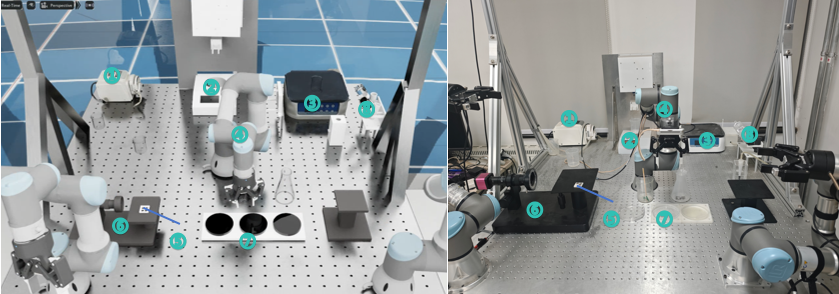
\includegraphics[width=\columnwidth]{images/sim and real.png}
    \caption{实验硬件平台及其在Isaac Sim中的仿真模型，展示了溶液配置、水滴角和梯度稀释工作站。标注组件如下：(1) 水泵——配置溶液时加水；(2) 电子秤——称量所需药品质量；(3) 摇床；(4) UR3机械臂——配置溶液、金属薄膜制备等操作；(5) 金属基材薄膜制备原材料；(6) 水滴角检测装置；(7) 培养皿——放置不同溶液；(8) 所需药品。}
    \label{fig:hardware_setup}
\end{figure}
\fi

\begin{table}[!t]
\renewcommand{\arraystretch}{1.3}
\caption{独立技能测试的虚实迁移IL成功率（非完整工作流）}
\label{tab:il_manipulation}
\centering
\resizebox{\columnwidth}{!}{
\begin{tabular}{lcccccc}
\hline\hline
\textbf{任务} & \multicolumn{2}{c}{\textbf{Vanilla BC}} & \multicolumn{2}{c}{\textbf{DR Only}} & \multicolumn{2}{c}{\textbf{本文方法（完整）}} \\ \hline
 & $n$/成功 & 成功率 & $n$/成功 & 成功率 & $n$/成功 & 成功率 \\
试剂移液 & 50\,/\,20 & 40.0\% & 50\,/\,33 & 66.0\% & 50\,/\,\textbf{42} & \textbf{84.0\%} \\
液滴滴加（水滴角） & 50\,/\,9 & 18.0\% & 50\,/\,29 & 58.0\% & 50\,/\,\textbf{40} & \textbf{80.0\%} \\
梯度稀释对准 & 50\,/\,14 & 28.0\% & 50\,/\,32 & 64.0\% & 50\,/\,\textbf{42} & \textbf{84.0\%} \\ \hline
\textbf{合并技能回合} & 150\,/\,43 & 28.7\% & 150\,/\,94 & 62.7\% & 150\,/\,\textbf{124} & \textbf{82.7\%} \\ \hline\hline
\end{tabular}
}
\end{table}

表\ref{tab:il_manipulation}中三种方法合并技能回合成功率的Wilson 95\%区间依次为[22.0,36.4]\%、[54.7,70.0]\%和[75.8,87.9]\%。本文方法在移液、滴加和稀释各50次测试中的区间分别为[71.5,91.7]\%、[67.0,88.8]\%和[71.5,91.7]\%。这些合并回合不是完整工作流，不能将82.7\%称为端到端成功率。

\subsubsection{补充虚实迁移验证方案}
\label{subsec:transfer_protocol}
为将技能迁移与材料实验可靠性联系起来，补充验证拟选择实际工作流中的精密操作，例如移液或定点滴加，对比仿真BC直接部署、BC加域随机化、以及域随机化加10次完整真实示范正则化微调。固定策略结构、仿真示范集、标称任务设置与测试预算，仅改变域随机化和真实数据微调。各方法采用匹配的初始条件集合，随机安排执行顺序，每次试验后重置工作台，并以多个训练或微调随机种子评估策略间差异。现有汇总表并不能证明这些控制条件和精度测量已经全部实施；本段为待执行的补充方案。

真实示范、验证集与实机测试回合相互独立，测试前冻结策略与验收阈值。初步计划每种方法、每个测试条件至少开展30次独立实机试验，最终样本量依据所需置信区间宽度和对比检验功效确定。报告回合在不同训练策略之间的分配；单个策略的重复试验不能反映训练随机性。

移液使用校准天平测量实际输出质量，按记录温度下的液体密度换算体积，报告有符号偏差、平均绝对相对体积误差及同一目标剂量的输出CV。定点滴加在标定平面上测量实际液滴中心与目标位置的距离；若任务也要求剂量精度，则单独测量剂量误差。预先规定各任务的体积或位置容差，仅当全部精度要求通过且无碰撞、非预期溢出或非计划人工介入时判定成功。保留所有失败回合，完成回合的精度与失败数同时报告，不得静默删除失败样本。报告成功次数/总次数、Wilson 95\%置信区间及精度指标的回合级不确定性。

\subsubsection{少样本效率}
\label{subsec:few_shot}

补充示范数量实验拟固定域随机化预训练策略，对比$M\in\{0,5,10,20\}$次完整真实示范，其中$M=0$为不进行真实微调的DR策略。一次示范指一次完整操作轨迹，而非一帧图像。从仅供训练的示范池构建嵌套子集，并重复子集抽样和不同随机种子的微调；各组使用相同的独立测试条件分布。超参数仅使用验证集选择，测试数据不得参与训练或模型选择。除精度与成功率外，还记录示范采集和微调耗时。该补充方案尚待执行，已有表格中的$M=50$行保留为原有汇总，不代表此次新增实验。

我们分析了真实世界演示数量$M$对微调性能的影响。表\ref{tab:few_shot}展示了不同$M$值的结果。

\begin{table}[!t]
\renewcommand{\arraystretch}{1.3}
\caption{少样本演示数量的影响}
\label{tab:few_shot}
\centering
\begin{tabular}{lccc}
\hline\hline
\textbf{演示数量 ($M$)} & \textbf{实验次数} & \textbf{成功次数} & \textbf{成功率 (\%)} \\ \hline
0 (DR Only) & 50 & 31 & 62.0 \\
5 & 50 & 39 & 78.0 \\
10 & 50 & \textbf{42} & \textbf{84.0} \\
20 & 50 & 42 & 84.0 \\
50 & 50 & 43 & 86.0 \\ \hline\hline
\end{tabular}
\end{table}

现有汇总在$M=10$时给出84.0\%成功率，但不足以确认最优示范数量或具有统计可靠性的性能平台期。作出上述结论前，需要说明具体任务、示范时长、训练随机种子，以及该批次与表\ref{tab:il_manipulation}中测试回合的关系。

\subsubsection{未见条件与泛化测试}
\label{subsec:transfer_generalization}
微调结束后冻结策略，分别测试标称条件、训练随机化范围内的新配置和超出训练范围的条件。优先改变物体初始位置、光照以及硬件兼容的容器尺寸，先开展单因素测试，并明确记录训练和测试的数值范围及真实示范的覆盖情况。只有同时未被仿真随机化和真实微调数据覆盖的条件，才能称为范围外条件；训练范围内的新样本仅证明分布内鲁棒性。实机测试不得超出已验证的硬件安全边界。

各方法和条件使用相同的试验预算与验收规则，报告精度、成功率、相对标称条件的性能变化及失败类别，不能仅以跨条件合并成功率代表泛化。该测试及其数值结果尚待完成，不从已有标称条件成功率推断泛化提升。后续完整薄膜流程保留策略版本与统一运行编号，将操作表现关联到流程成功及薄膜质量，检验精密操作改善是否能转化为合格薄膜产出率的提升。

\subsection{浸涂薄膜制备与材料质量评估}
\label{subsec:exp_dipcoat_quality}

% 按作者要求暂时隐藏原图7及其正文引用。
\iffalse
图~\ref{fig:thin_film_sequence}展示了薄膜处理工作流中机械臂操作干燥烘箱的过程。
\begin{figure*}[!t]
    \centering
    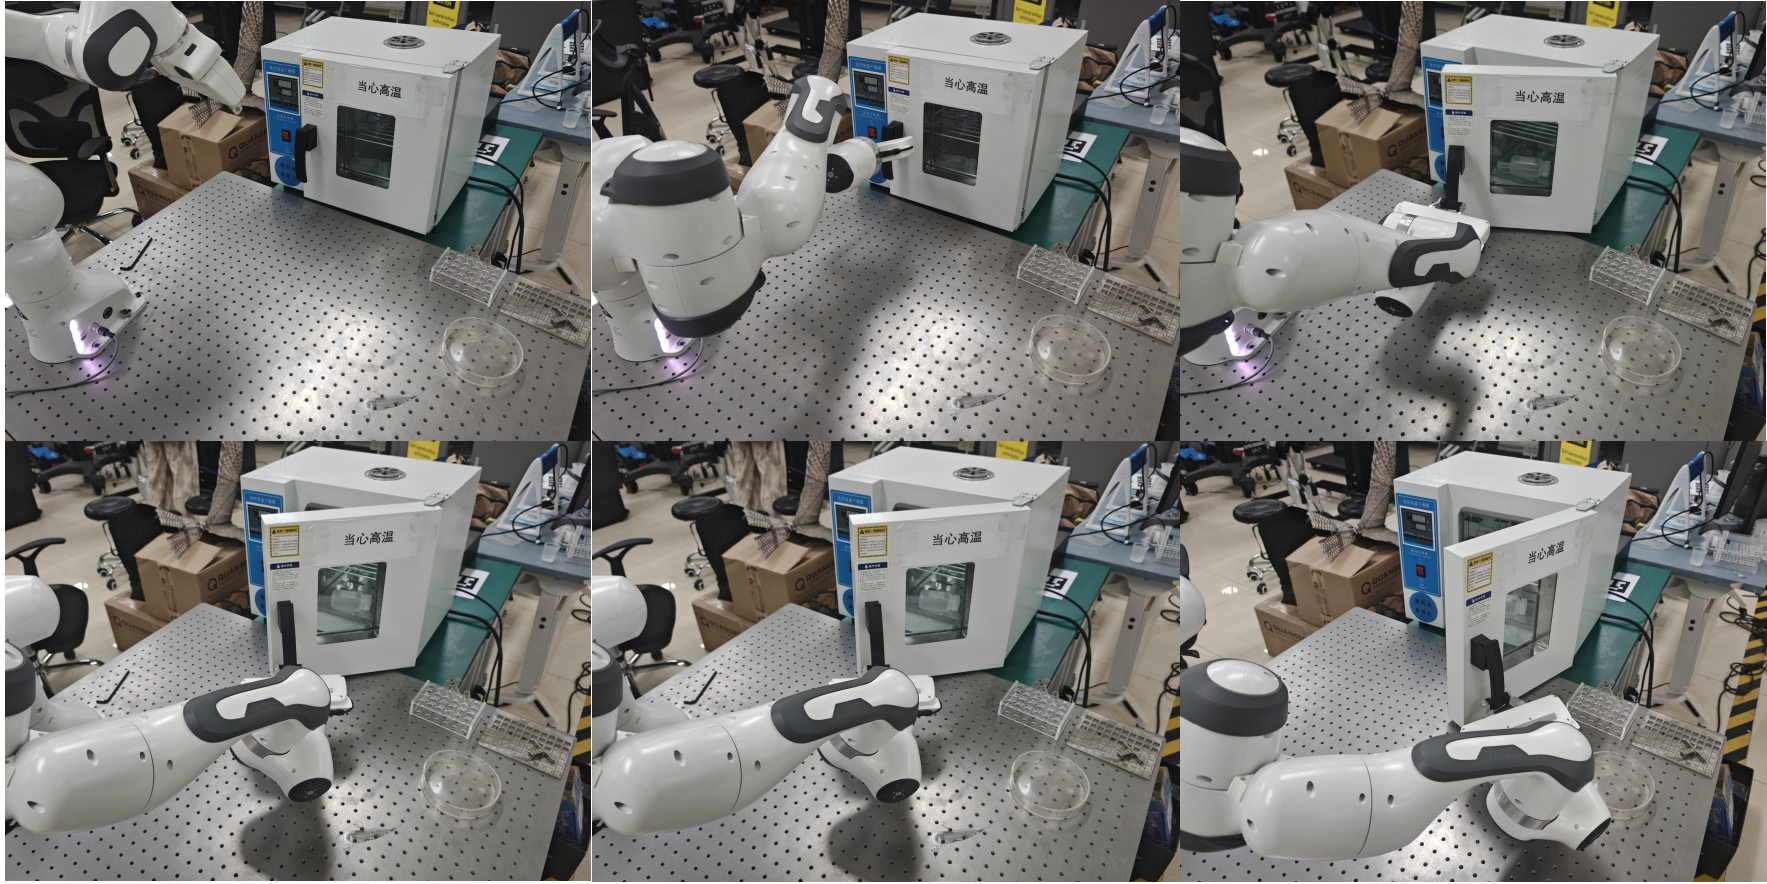
\includegraphics[width=0.9\textwidth]{images/thin_film.png}
    \caption{薄膜处理工作流中的烘箱操作序列，按上排从左到右、再下排从左到右的顺序阅读。图中展示了机械臂接近烘箱、操作门把手及打开烘箱的过程。}
    \label{fig:thin_film_sequence}
\end{figure*}
\fi
已完成的浸涂实验应以材料质量而非仅以机械臂动作成功进行评价。在同一前驱液批次、基底预处理、浸入深度、停留时间、目标提拉速度、干燥/固化条件和测量时间下，比较受训实验人员手工浸涂、机器人固定轨迹与本文学习控制三组。基底应随机分组；条件允许时，材料表征人员应不知道样品所属组别。统计样本量是独立基底数，而非同一基底上的测量点数。

在每片基底的预设位置测量膜厚，以$\mathrm{CV}_{h,i}=100s(h_{ij})/\bar h_i$表示片内膜厚变异系数，并同时报告平均膜厚$\bar h_i$。在规定液滴体积和滴加后等待时间下测量多个位置的静态水接触角，报告均值及空间标准差。采用轮廓仪或AFM，在固定扫描面积内测量表面粗糙度$R_a$或$R_q$。耐腐蚀性测试应统一电解液、暴露面积、温度、稳定时间及电化学流程，报告极化拟合所得腐蚀电流密度$i_{\mathrm{corr}}$；如有EIS数据，再报告低频阻抗$|Z|_{0.01\,\mathrm{Hz}}$。薄膜成功标准应事先按均匀性、附着力与缺陷阈值定义，不能仅凭目视判断。

\begin{table*}[!t]
\renewcommand{\arraystretch}{1.2}
\caption{人工、固定轨迹与学习控制的薄膜质量对比。待取得实测值后填写；不能根据机器人任务成功率推断材料质量。}
\label{tab:film_quality}
\centering
\begin{tabular}{lcccccc}
\hline\hline
\textbf{执行方式} & \textbf{基底数$n$} & \textbf{平均膜厚} & \textbf{膜厚CV (\%)} & \textbf{接触角 ($^\circ$)} & \textbf{粗糙度$R_a$} & \textbf{$i_{\mathrm{corr}}$} \\ \hline
人工操作 & 待填 & 待填 & 待填 & 待填 & 待填 & 待填 \\
机器人固定轨迹 & 待填 & 待填 & 待填 & 待填 & 待填 & 待填 \\
学习控制（本文） & 待填 & 待填 & 待填 & 待填 & 待填 & 待填 \\ \hline\hline
\end{tabular}
\end{table*}

最终表格应补充单位、基底层面的均值$\pm$标准差和95\%置信区间。如有低频阻抗或其他独立防护指标，也应同时报告。三组比较应按数据分布与独立基底设计预先选定统计检验，并对两两比较进行多重检验校正。由于本轮修订尚未获得具体实测值，此处不宣称学习控制在薄膜质量或耐腐蚀性能方面优于基线。

% 跨平台交接实验保留为独立待补内容。

% TODO: 添加跨平台交接实验

% TODO: 添加浸涂质量和交接序列图片
% \begin{figure}[htbp]
%     \centering
%     \includegraphics[width=\columnwidth]{images/dip_coating_results.png}
%     \caption{浸涂薄膜制备的定性结果。}
%     \label{fig:dip_coating_results}
% \end{figure}

% \begin{figure}[htbp]
%     \centering
%     \includegraphics[width=\columnwidth]{images/handover_sequence.png}
%     \caption{基于ArUco定位的跨平台交接序列。}
%     \label{fig:handover_sequence}
% \end{figure}
% ==================== END TODO ====================

% ==================== TODO: P2 - 训练曲线与消融实验（1天） ====================
\subsection{训练收敛与消融研究}
\label{subsec:exp_training_ablation}

% TODO: 添加DRL训练曲线（奖励 vs 迭代次数）
% - 基线PPO vs 姿态感知PPO收敛对比
% - 奖励分解（距离、抓取、抬升、碰撞惩罚）

% \begin{figure}[htbp]
%     \centering
%     % \includegraphics[width=\columnwidth]{images/drl_training_curve.png}
%     \caption{DRL训练收敛曲线。基线PPO与姿态感知PPO的奖励随训练迭代的变化对比。}
%     \label{fig:drl_training_curve}
% \end{figure}

% TODO: 添加IL训练曲线（损失 vs 轮次）
% - 仿真中BC损失收敛
% - 真实示教少样本微调损失

% \begin{figure}[htbp]
%     \centering
%     % \includegraphics[width=\columnwidth]{images/il_training_curve.png}
%     \caption{IL训练损失曲线。仿真中的行为克隆损失与真实世界少样本微调的收敛过程。}
%     \label{fig:il_training_curve}
% \end{figure}

% TODO: 添加消融实验表——各组件贡献
% ==================== END TODO ====================

% ==================== TODO: P2 - SOTA对比（1-2周） ====================
\subsection{与最先进方法的对比}
\label{subsec:exp_sota}

% TODO: 添加SOTA对比表

% TODO: 添加雷达图或多维对比柱状图
% \begin{figure}[htbp]
%     \centering
%     \includegraphics[width=\columnwidth]{images/sota_comparison.png}
%     \caption{与最先进实验室自动化系统的多维度对比。}
%     \label{fig:sota_comparison}
% \end{figure}
% ==================== END TODO ====================

\subsection{端到端自主工作流集成}
\label{subsec:exp_end_to_end}

\subsubsection{失败分类}
每次失败应根据首个未恢复原因赋予唯一主类别：感知、抓取、移液、对接/交接、运输/溢出、通信或恢复次数耗尽。其他促成因素可作为次要标签。按工作流报告各类别失败次数、占全部失败的比例、成功恢复次数及损失时间，避免一次失败重复计数。现有汇总表不足以完成此分析，需逐回合日志。

\subsubsection{科学结果质量与统计检验}
机器人动作完成和实验产物合格应分开报告。溶液制备应报告独立配液的目标/实测浓度误差及移液变异系数（CV）；梯度稀释应报告名义与实测浓度的线性拟合斜率、$R^2$、各级相对误差及阴性对照交叉污染率；薄膜按表\ref{tab:film_quality}报告膜厚CV、接触角偏差、粗糙度与耐腐蚀指标。所有合格阈值须在比较各组结果前确定，并报告同时满足各项阈值的独立运行比例。

关键二元比较应列出成功次数、总次数和Wilson 95\%区间；独立回合可采用双侧Fisher精确检验，配对场景应采用相应的配对精确检验。连续质量指标报告效应量和按独立回合或基底聚类的bootstrap 95\%区间，多组两两比较需作多重检验校正。未获得原始记录前不填写$p$值或伪造聚类置信区间。

为单独检验失败恢复编排的作用，后续应在相同低层技能、初始条件与注入故障下比较：（1）任一状态条件失败即终止的固定顺序状态机；（2）允许有限次数恢复的本文分层状态机。故障应包括抓取失败、对接偏差和过期感知数据。报告试验次数、完整工作流成功率、各阶段失败与恢复率、重试次数、人工干预次数及完成时间。下文现有结果不包含这一消融实验，因此不能用于证明分层状态机优于固定顺序执行。

完整工作流应以同一运行编号从开始追踪到结束，任一阶段失败不得重置分母。分别定义：（1）溶液制备：取试剂、定量配液、混合及质量检测；（2）薄膜制备：溶液送达、基底处理、浸涂、固化及薄膜质量验收；（3）梯度稀释：试剂送达、吸头管理、稀释及浓度/污染检测。仅当全部步骤与科学质量阈值均合格且无计划外人工干预时，才计为完整成功；分别报告首次成功率与恢复后成功率。

下表现有次数是各操作阶段的独立汇总，不能相乘、相加或视为完整流程结果。尤其若均指同一批50次运行，原稿“全循环42/50”与水滴角阶段40/50在逻辑上冲突，须先核对逐回合日志。原稿“连续成功10次”也须有可追溯的运行编号，本次不作为已核实的独立结果。

\begin{table}[!t]
\renewcommand{\arraystretch}{1.3}
\caption{现有阶段级计数；完整工作流结果需逐回合日志核对}
\label{tab:end_to_end}
\centering
\begin{tabular}{lccc}
\hline\hline
\textbf{工作流阶段} & \textbf{实验次数} & \textbf{成功次数} & \textbf{成功率 (\%)} \\ \hline
自主转移 & 50 & 44 & 88.0 \\
直立抓取 & 50 & 43 & 86.0 \\
试剂移液 & 50 & 42 & 84.0 \\
水滴角测量 & 50 & 40 & 80.0 \\
梯度稀释 & 50 & 42 & 84.0 \\ \hline
\textbf{完整工作流} & \textbf{待核对} & \textbf{待核对} & \textbf{待核对} \\ \hline\hline
\end{tabular}
\end{table}

\begin{table}[!t]
\caption{完整工作流结果填写模板（独立运行）}
\label{tab:workflow_complete}
\centering
\begin{tabular}{lccc}
\hline\hline
\textbf{流程} & \textbf{运行数} & \textbf{首次成功} & \textbf{恢复后成功} \\ \hline
溶液制备 & 待填 & 待填 & 待填 \\
薄膜制备 & 待填 & 待填 & 待填 \\
梯度稀释 & 待填 & 待填 & 待填 \\ \hline\hline
\end{tabular}
\end{table}

% \begin{figure*}[!t]
%     \centering
%     % \includegraphics[width=\textwidth]{figures/end_to_end_snapshots.png}
%     \caption{自主三阶段实验室工作流的顺序快照：(a)--(b) 直立器材抓取和试剂移液；(c)--(d) 约束感知转移和用于水滴角检测的液滴滴加；(e)--(f) 高精度梯度稀释和微孔板对准。}
%     \label{fig:sequential_snapshots}
% \end{figure*}

\section{结论与未来工作}
\label{sec:conclusion}

\subsection{结论}
\label{subsec:conclusion_summary}
在本文中，我们提出了一种多平台混合机器人框架，专为复杂生化实验室工作流的端到端自动化量身定制，具体涵盖溶液配置、水滴角测量和用于生物培养的梯度稀释。通过解耦控制架构，我们的系统通过约束感知的经典运动规划保证了宏观移动底盘导航过程中的绝对流体稳定性。对于灵巧的、接触密集型的机械臂操作，我们实施了一种混合学习策略：在Isaac Sim中训练的姿态感知大规模并行深度强化学习（DRL）智能体用于直立器材抓取，以及带有正则化少样本真实世界微调的遥操作引导模仿学习（IL）策略用于精密微量移液和液滴滴加。大量的实证评估表明，我们的框架在所报告操作技能的合并回合中达到82.7\%的成功率，有效地消除了自主实验室中物理试错的高昂成本和风险。

\subsection{局限性与未来工作}
\label{subsec:limitations_future}
尽管取得了令人鼓舞的结果，但仍存在一些局限性。目前，模仿学习的示教获取依赖于手动遥操作，当扩展到数百种不同的化验协议时，这可能成为瓶颈。此外，视觉策略主要针对刚性玻璃药瓶和微孔板进行了优化，需要进一步适应高度可变形的器材或软组织。

所提供的状态同步汇总值满足预设目标，但仍需回合数、原始轨迹、独立参考测量和不确定性区间来核验精度。

在未来的工作中，我们计划将视觉语言模型（VLM）和大语言模型（LLM）集成到机器人系统中。这将使系统能够语义解析高级自然语言指令（例如"准备1:10的梯度稀释系列并测量基底水滴角"），并自动生成分层状态机（HSM）序列和控制基元，从而更接近完全自主的科学发现。


% ==================== 参考文献 ====================
\begin{thebibliography}{99}

\bibitem{burger2020mobile}
B. Burger 等, ``移动机器人化学家,'' \textit{Nature}, vol. 583, no. 7815, pp. 237--241, 2020.

\bibitem{macleod2020self}
B. P. MacLeod 等, ``用于加速薄膜材料发现的自动驾驶实验室,'' \textit{Science Advances}, vol. 6, no. 20, p. eaaz8867, 2020.

\bibitem{dt_migration_mobile}
Y. Wang 和 X. Zhao, ``工业移动机器人的数字孪生动态迁移方法,'' \textit{Robotics and Computer-Integrated Manufacturing}, vol. 92, p. 102864, 2025.

\bibitem{dt_port_inspection}
H. Jiang, Z. Guo, 和 Z. Zhang, ``智能港口巡检机器人的数字孪生与路径规划,'' \textit{Journal of Marine Science and Engineering}, vol. 14, no. 2, p. 186, 2026.

\bibitem{dt_unity_ros}
D. Kawshan 和 Q. Peng, ``基于Unity-ROS集成的机器人路径规划与实时执行数字孪生框架：系统架构与实验验证,'' \textit{Machines}, vol. 14, no. 4, p. 387, 2026.

\bibitem{makoviychuk2021isaac}
V. Makoviychuk 等, ``Isaac Gym：基于高性能GPU的机器人学习物理仿真,'' in \textit{NeurIPS Datasets and Benchmarks}, 2021.

\bibitem{dt_collision_timeseries}
F. El Kalach, M. A. Farahani, P. Samaha 等, ``基于时间序列预测的数字孪生机器人碰撞检测,'' \textit{Journal of Intelligent Manufacturing}, pp. 1--18, 2026.

\bibitem{dt_vr_collaboration}
A. Cimino, F. Longo, L. Nicoletti 等, ``结合仿真与虚拟现实实现协作人机工作空间的互操作数字孪生,'' \textit{International Journal of Production Research}, vol. 63, no. 23, pp. 9465--9501, 2025.

\bibitem{dt_task_replanning}
X. Li, B. He, Z. Wang 等, ``用于机器人操作任务重规划与人机控制的数字孪生系统,'' \textit{Advanced Engineering Informatics}, vol. 62, p. 102570, 2024.

\bibitem{mandlekar2021matters}
A. Mandlekar 等, ``从离线人类演示中学习机器人操作的重要因素,'' in \textit{Conf. on Robot Learning (CoRL)}, pp. 1678--1690, 2021.

\bibitem{johannink2019residual}
T. Johannink 等, ``用于机器人控制的残差强化学习,'' in \textit{Proc. IEEE Int. Conf. Robot. Autom. (ICRA)}, pp. 6023--6029, 2019.

\bibitem{szymanski2022automated}
N. J. Szymanski 等, ``用于加速新材料合成的自主实验室,'' \textit{Nature}, vol. 624, pp. 86--91, 2023.

\bibitem{ho2016gail}
J. Ho and S. Ermon, ``Generative adversarial imitation learning,'' in \textit{Adv. Neural Inf. Process. Syst. (NeurIPS)}, vol. 29, 2016.

\end{thebibliography}

\end{document}
